%
% Copyright (c) 2008 Betti "Osterholz
%
% Permission is granted to copy, distribute and/or modify this document
% under the terms of the GNU Free Documentation License, Version 1.2 or
% any later version published by the Free Software Foundation;
% with no Invariant Sections, no Front-Cover Texts, and no Back-Cover Texts.
%
% A copy of the license is included in the file ``fdl.tex'' .
%

%Pfad fuer Bilder
\graphicspath{{./material_enviroment_implementation/}}
\graphicspath{{./material_enviroment_implementation/}{../material_enviroment_implementation}}


\newpage
\part{Implementation des genetische Algorithmus}
\label{partImplementationAlgorithmus}

In diesem Teil wird der Implementationsentwurf des genetischen Algorithmus vorgestellt. Dazu geh"oren die Klassenhierarchien und die Schnittstellenbeschreibungen. Die Schnittstellenbeschreibungen geschieht in pseudo C++.

Der genetische Algorithmus wird dem separaten Namensraum mit dem Namen ``enviroment'' zugeordnet. Er wird generisch (bzw. allgemein) implementiert, so dass er auch f"ur andere Anwendungen au"ser Fib verwendet werden kann. In Abbildung \ref{figEnviromentAlgorithmus} ist eine Ablaufskizze des genetischen Algorithmus dargestellt.

Des Weiteren wird in diesem Abschnitt auch der allgemeine Entwurf f"ur die Operatoren vorgestellt, da der genetische Algorithmus nur schwer von diesen getrennt gesehen werden kann.


\begin{figure}[htbp]
\begin{center}
  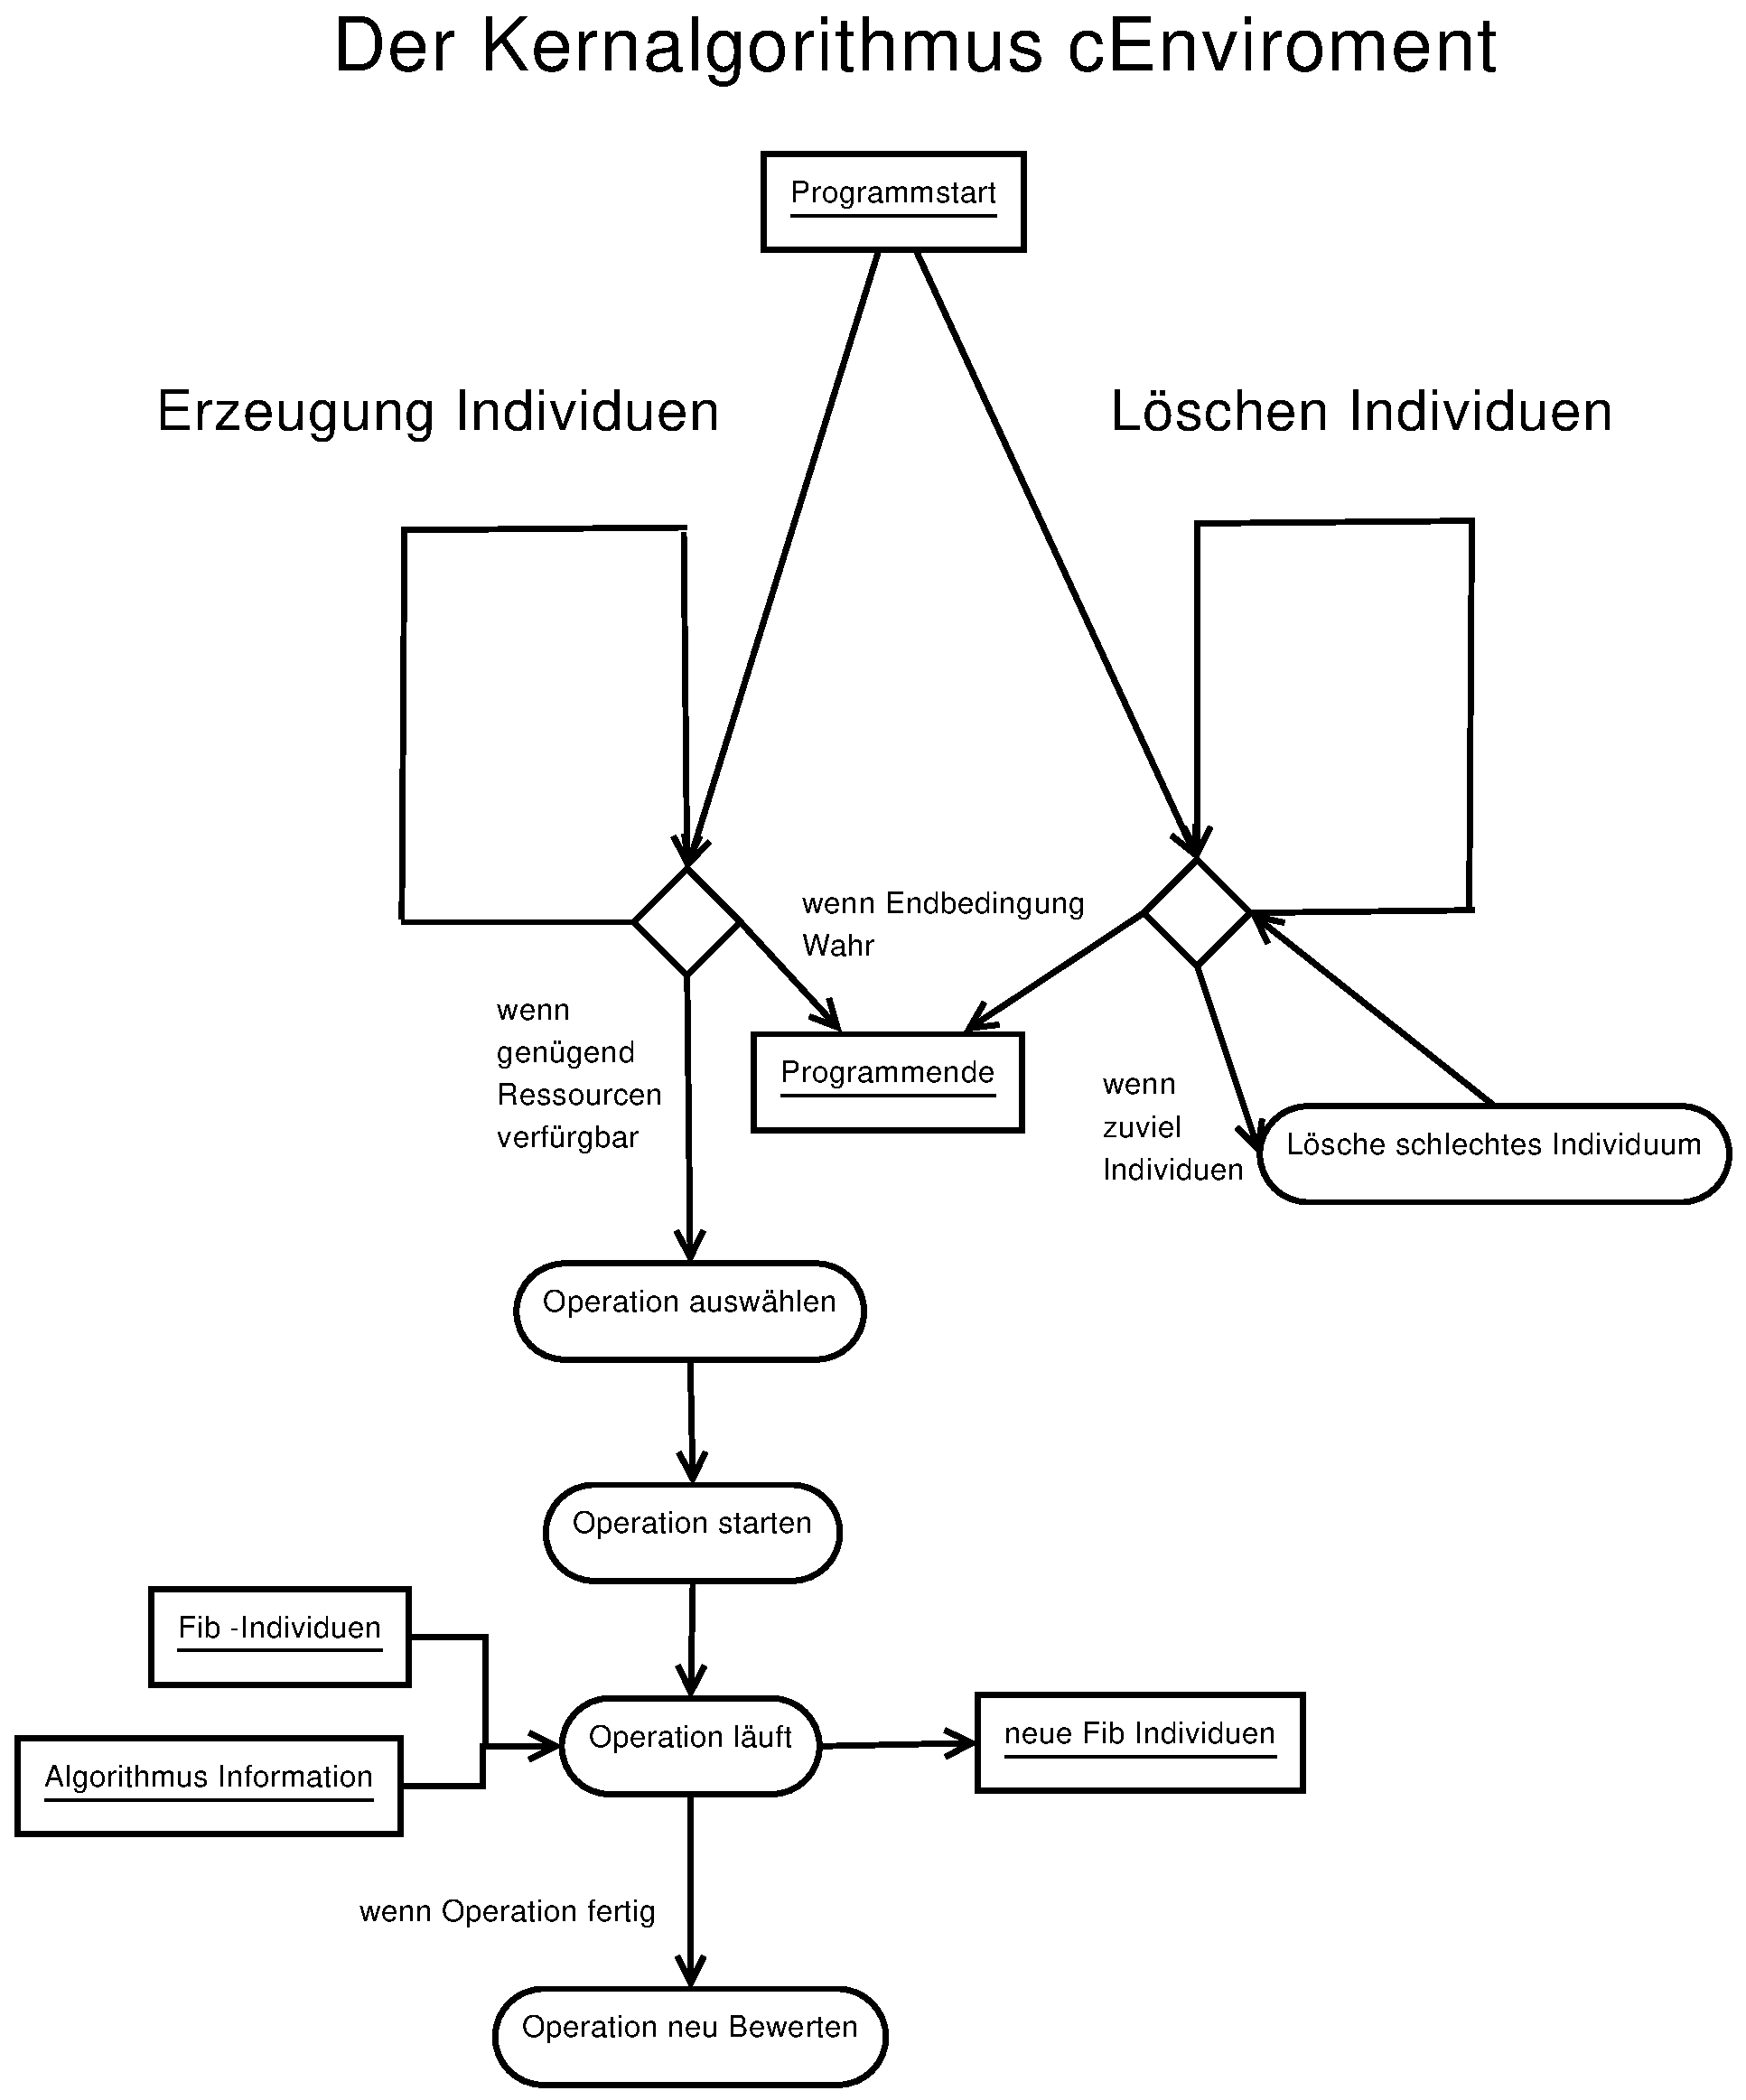
\includegraphics[scale=0.4]{programmablauf}
\end{center}
\caption{Ablaufdiagramm des genetischen Algorithmus}
\label{figEnviromentAlgorithmus}
\end{figure}


\section{Hilfsmethoden}

Hilfsmethoden, die bei der Implementierung hilfreich sind, aber nicht zur eigentlichen Schnittstelle geh"oren, werden nach Bedarf implementiert, hier aber nicht aufgef"uhrt. Sie sollten nach M"oglichkeit von au"sen nicht zugreifbar sein (also \verb|privat| oder \verb|protected| deklariert sein).


\section{Copyright}

Der genetische Algorithmus wird unter die GPL (siehe Abschnitt \ref{secGPL} auf Seite \pageref{secGPL}) gestellt. Er kann also frei angepasst, ver"andert und eingebunden werden, solange das Ergebnis wieder unter der GPL steht. Da der genetische Algorithmus als eigenst"andiges Programm zu sehen ist, sollten die zus"atzlichen Freiheiten der LGPL (siehe Abschnitt \ref{secLGPL} auf Seite \pageref{secLGPL}) f"ur ihn nicht n"otig sein.


\section{Allgemeine Regeln}

F"ur die Implementation des genetischen Algorithmus gibt es ein paar allgemeine Regeln:
\begin{itemize}
 \item Der Algorithmus ist so zu modularisieren, dass Module einfach ausgetauscht werden k"onnen, um ihn an andere Problemstellungen m"oglichst leicht anzupassen zu k"onnen.
 \item Nur der Kernalgorithmus kann Individuen l"oschen.
 \item Nur der Algorithmus bewertet die Operatoren.
 \item Nur der Algorithmus kann eine Operation zum Erzeugen neuer Individuen starten.
 \item Nur der Algorithmus entscheidet, wann er fertig ist und beendet sich. Er kann dabei aber auch auf Signale von au"sen reagieren.
\end{itemize}



\section{Module}

Um den Algorithmus so allgeimein wie m"oglich zu implementieren, werden einige Funktionen von externen Modulen bzw. Klassen realisiert. Im Nachfolgenden werden diese Module vorgestellt.

\subsection{Modul f"ur die Individuen}

Die Individuen sind die zentralen Objekte im Algorithmus. Um verschiedene Problemstellungen bearbeiten zu k"onnen, m"ussen Individuen an die jeweile Problemstellung angepasst werden k"onnen. N"aheres dazu in Abschnitt \ref{secIndividual} auf Seite \pageref{secIndividual}.


\subsection{Modul f"ur die Initialisierung}

Bei Start des Algorithmus (Programmstart) sind einige Aufgaben auszuf"uhren. Dazu geh"ort beispielsweise, dass ein Individuum erzeugt und in die Individuenpopulation (bzw. Individuenliste) als erstes Individuum eingef"ugt wird. N"aheres dazu in Abschnitt \ref{secInitAlgoritmus} auf Seite \pageref{secInitAlgoritmus}.


\subsection{Module f"ur Entscheidungen}

Diese Module werden verwendet, wenn etwas entschieden werden soll. Sie enthalten im Allgemeinen nur eine Funktion, mit der eine Bedingung gepr"uft werden kann.


\subsubsection{Modul f"ur die Ressourcenpr"ufung}

Dieses Modul ist daf"ur zust"andig zu pr"ufen, ob genug System-/Rechnerressourcen vorhanden sind, um weitere Operationen zu starten und auszuf"uhren. N"aheres dazu in Abschnitt \ref{secResourceCheck} auf Seite \pageref{secResourceCheck}.

"Uber das Modul zum Ausw"ahlen einer Operation werden dann neue Operationen gestartet, wenn genug Ressourcen vorhanden sind.


\subsubsection{Modul f"ur die Endbedingung}

Das Modul zum Pr"ufen der Endbedingung zeigt an, wann die Endbedingung erf"ullt ist und der Algorithmus beendet werden soll. N"aheres dazu in Abschnitt \ref{secEndConditionCheck} auf Seite \pageref{secEndConditionCheck}.


\subsubsection{Modul f"ur die maximale Populationsgr"o"se}

Damit die Populationsgr"o"se nicht in das Unendliche anw"achst, muss diese beschr"ankt werden. Um zu bewerten, wann ``zuviele Individuen'' vorhanden sind, dient das Modul f"ur die maximale Populationsgr"o"se. N"aheres dazu in Abschnitt \ref{secMaxPopulation} auf Seite \pageref{secMaxPopulation}.

Das L"oschen von Individuen, um die Population zu beschr"anken, geschieht allerdings mit dem Modul zum L"oschen von Individuen.


\subsection{Module f"ur Vorg"ange}

Die folgenden Module dienen dazu, bestimmte Vorg"ange oder Aufgaben auszuf"uhren bzw. zu erf"ullen.


\subsubsection{Modul zum Bewerten eines Individuums}

Um Individuen vergleichen zu k"onnen, m"ussen diese bewertet werden. Dazu dient das Modul zum Bewerten von Individuen. Jedes neu erzeugte Individuum sollte bewertet werden. Diese Bewertung ist dann zum Individuum zu speichern. Das bedeutet, dass dieses Modul aus zwei Teilen besteht: dem Bewerter und der Bewertung f"ur Individuen.

Mehr zur Bewertung im Abschnitt \ref{secCObjectFitness} auf Seite \pageref{secCObjectFitness} und zum Bewerter im Abschnitt \ref{secCObjectFitnessAlgorithm} auf Seite \pageref{secCObjectFitnessAlgorithm}.


\subsubsection{Modul zum Ausw"ahlen eines guten Individuums}

Einige Operatoren werden Informationen aus bereits existierenden Individuen nutzen wollen, um neue Individuen zu erzeugen. Damit die Individuen unabh"angig von der nachfragenden Operation gew"ahlt werden, ist die Wahl in einem seperaten Modul im Algorithmus zu implementieren. Dieses Modul sollte gute Individuen bevorzugen und austauschbar sein, um auch andere Wahlstrategien leicht einsetzen zu k"onnen. Davon unabh"angig k"onnen Operationen nat"urlich ihre eigenen Wahlmechanismen implementieren.

N"aheres dazu in Abschnitt \ref{secIndividualSelection} auf Seite \pageref{secIndividualSelection}.


\subsubsection{Modul zum L"oschen von Individuen}

Wenn die maximale Populationsgr"o"se "uberschritten ist, m"ussen existierende Individuen gel"oscht werden. Die Auswahl der zu l"oschenden Individuen geschieht "uber ein austauschbares Modul. Die L"oschoperation selbst wird im Kernalgorithmus ausgef"uhrt, um zu vermeiden, dass externe Module "uber eine Schnittstelle Individuen l"oschen k"onnen.

Im Abschnitt \ref{secIndividualDeletionSelection} auf Seite \pageref{secIndividualDeletionSelection} wird dieses Modul beschrieben.


\subsubsection{Modul zum Bewerten einer Operation}

Um zu bestimmen, wie gut Operatoren in bestimmten Situationen arbeiten, m"ussen die Operatoren anhand ihrer Leistung bewertet werden. Da die Art der Operatoren und damit die Bewertungskriterien sich "andern k"onnen, muss dieses Modul austauschbar sein.

Das Modul zum Bewerten von Operatoren wird im Abschnitt \ref{secCOperationFitnessAlgorithmus} auf Seite \pageref{secCOperationFitnessAlgorithmus} beschrieben.


\subsubsection{Modul zum Ausw"ahlen einer Operation}

Um neue Individuen zu erzeugen, m"ussen Operatoren ausgew"ahlt werden. Da die Art der Operatoren sich "andern kann, muss dieses Modul austauschbar sein.

Dieses Modul wird im Abschnitt \ref{secCChoosOperator} auf Seite \pageref{secCChoosOperator} beschrieben.


\section{Inividuen cIndividual}\label{cIndividual}
\label{secIndividual}

Der Algorithmus arbeitet auf der Basis von Individuen. Deshalb sind diese von zentraler Bedeutung f"ur den Algorithmus. Individuen sind es, die er schlie"slich verbessern soll, und das Ergebnis des Algorithmus soll auch ein Individuum sein. Deshalb sind Individuen von zentraler Bedeutung f"ur den Algorithmus.

Die Klasse \verb|cIndividual| repr"asentiert ein Individuum in einer abstrakten Form. Dabei h"alt sie nicht nur die Informationen eines vollst"andigen Objekts, welches verbessert werden soll, sondern auch weitere Angaben. Mit diesen Angaben soll eine beschleunigte Verarbeitung von Individuen erm"oglicht werden.

\bigskip\noindent
Zu den Informationen, welche die Klasse \verb|cFibIndividual| bereitstellt, geh"oren:
\begin{itemize}
 \item das Objekt, welches das Individuum repr"asentiert.
 \item Zusatzinformationen zu einem Individuum \verb|cIndividualInfo| (Siehe Abschnitt \ref{secCIndividualInfo} auf Seite \pageref{secCIndividualInfo})
\end{itemize}


\subsection{Schnittstellenbeschreibung}

\subsubsection{cIndividual}

\textbf{Syntax:} \verb|cIndividual( void * pObject,| \\\verb| const cIndividualInfo & individualInfo )| \\

Der Konstruktor f"ur ein Indiviuum; er erzeugt ein Individuum.

Weder von \verb|pObject| noch von \verb|individualInfo| werden Kopien angefertigt. Beide Objekte werden direkt f"ur das Individuum verwendet.

\bigskip\noindent
\textbf{Eingabeparameter:}
\begin{itemize}
 \item \verb|pObject|: Einen Zeiger auf das Objekt, welches das Individuum repr"asentieren soll.
 \item \verb|individualInfo|: Eine Refernz, auf die Zusatzinformationen f"ur das Objekt.
\end{itemize}

\bigskip\noindent
\textbf{R"uckgabe:} keine


\subsubsection{equal}\index{cIndividual!equal()}\index{cIndividual!Gleichheit}\index{equal()}

\textbf{Syntax:} \verb|boolen equal( const cIndividual &individuum,| \\\verb| bool bCheckIdentifiers=true )| \\
oder \verb|bool operation==( const cIndividual &individuum )|

\bigskip\noindent
Diese Methoden pr"ufen, ob das aktuelle und "ubergebene Individuum gleich sind.

\bigskip\noindent
\textbf{Eingabeparameter:}
\begin{itemize}
 \item \verb|individuum|: Das Individuum, welches gleich zum aktuellen Individuum sein soll.
 \item \verb|bCheckIdentifiers|: Dieser Wert gibt an, ob bei der Gleichheitspr"ufung die beiden Identifier der Objekte (\verb|cIndividualIdentifier| und \verb|cOperationIdentifier|) mit ber"ucksichtigt werden sollen. Wenn er \verb|true| (=wahr) ist, werden die Identifier bei der Pr"ufung mit ber"ucksichtigt. Sonst, wenn er \verb|false| (=falsch) ist, werden die Identifier bei der Pr"ufung nicht ber"ucksichtigt. Es werden dann nur die Strukturen der Individuen auf Gleichheit gepr"uft. Standardwert ist \verb|true| (=wahr), womit auch die Identifier bei der Pr"ufung ber"ucksichtigt werden.
\end{itemize}

\bigskip\noindent
\textbf{R"uckgabe:} Die Methode gibt \verb|true| (=wahr) zur"uck, wenn das aktuelle Individuum gleich dem "ubergebenen Individuum ist, sonst \verb|false| (=falsch).


\subsubsection{getObjekt}\index{cIndividual!getObjekt()}\index{getObjekt()}

\textbf{Syntax:} \verb|void * getObject()|

\bigskip\noindent
Diese Methode gibt einen Zeiger auf das Objekt des Individuums zur"uck. Das Objekt ist der eigentliche Gegenstand des Algorithmus. Auf dem Individuum arbeiten die Operatoren. Das Objekt ist das, was ``verbessert'' werden soll. Die anderen Informationen des Individuums dienen nur dazu, dem Algorithmus Zusatzinformationen zum Objekt zu liefern und die Abarbeitung zu beschleunigen.

\bigskip\noindent
\textbf{Eingabeparameter:} keine

\bigskip\noindent
\textbf{R"uckgabe:} Eine Referenz auf das Objekt des Individuums.


\subsubsection{getInfo}\index{cIndividual!getInfo()}\index{getInfo()}

\textbf{Syntax:} \verb|cIndividualInfo * getInfo()|

\bigskip\noindent
Diese Methode liefert einen Zeiger auf die Zusatzinformationen des Individuums zur"uck. Dies sind Informationen zum Objekt des Individuums, welche dem Algorithmus und den Operatoren die Arbeit erleichtern. Sie enthalten auch allgemeine Informationen (wie z. B. die Erzeugungszeit des Objekts).

\bigskip\noindent
\textbf{Eingabeparameter:} keine

\bigskip\noindent
\textbf{R"uckgabe:} Einen Zeiger auf die Zusatzinformationen des Individuums.


\subsubsection{getClassName}\index{cIndividual!getClassName()}\index{getClassName()}

\textbf{Syntax:} \verb|string getClassName() const|

\bigskip\noindent
Diese Funktion gibt den Klassennamen ''cIndividual`` des Individuumobjekts zur"uck.

In abgeleiteten Klassen sollte diese Methode immer "uberschrieben werden, so dass der jeweilige Klassenname zur"uckgegeben wird.

\bigskip\noindent
\textbf{Eingabeparameter:} keine

\bigskip\noindent
\textbf{R"uckgabe:} Den Klassennamen ''cIndividual`` des Individuumobjekts.



\section{Zusatzinformationen zu einem Individuum cIndividualInfo}
\label{secCIndividualInfo}

Die Klasse \verb|cIndividualInfo| stellt zus"atzliche Informationen zu einem Individuum (bzw. Objekt) bereit.

\bigskip\noindent
Zu den Informationen, welche die Klasse \verb|cIndividualInfo| bereitstellt, geh"oren:
\begin{itemize}
 \item ein Wahrheitswert (boolean), der angibt, ob das Individuum noch lebt bzw. ob das Objekt noch existiert oder es tot ist, bzw. das Objekt gel"oscht wurde. Die Klasse \verb|cIndividualInfo| kann noch "uber das Ableben/ L"oschen des Individuums hinaus leben, um beispielsweise sp"atere statistiche Auswertungen zu erlauben.
 \item ein Identifier \verb|cIndividualIdentifier| f"ur das Individuum. Dies ist eine eindeutige nat"urliche Zahl f"ur das Inividuum und eine Zahl f"ur die genetischen Algorithmusinstanz, in dem es erzeugt wurde. Die genetische Algorithmusinstanz ben"otigt einen seperaten Identifier, da es vorgesehen ist, dass Individuen zwischen genetischen Algorithmusinstanzen migrieren k"onnen (zur Klasse \verb|cIndividualIdentifier| siehe Abschnitt \ref{secCIndividuumIdentifier} auf Seite \pageref{secCIndividuumIdentifier}).
 \item die Fitness des Objekts (zur Klasse \verb|cObjectFitness| siehe Abschnitt \ref{secCObjectFitness} auf Seite \pageref{secCObjectFitness}).
 \item der (lokale) Zeitpunkt der Erzeugung des Objekts.
 \item die Anzahl der bisher vom Algorithmus ausgef"uhrten Operationen.
 \item eine Liste mit den Identifieren der direkten Vorfahren des Inividuums. Diese k"onnen beispielsweise f"ur Heuristiken interessant sein.
 \item der Operatorname der Operation, mit der das Objekt erzeugt wurde, inklusive einem freien Feld (eine Unicodezeichenkette), in dem vom Operator weitere Eintr"age vorgenommen werden k"onnen. In dem freien Feld kann beispielsweise von der Operation eingetragen werden, welche Unteroperatoren sie mit welchen Parametern zur Erzeugung des Objekts benutzt hat. Diese Informationen (Name und freies Feld) werden als zwei Zeichenketten abgespeichert.
 \item der Identifier \verb|cOperationIdentifier| der erzeugenden Operation.
 \item der zur Erzeugung ben"otigte Aufwand $A$ (als Systemunab"ahngige Gleitkommazahl). Dieser wird in Abschnitt \ref{secOperationCost} auf Seite \pageref{secOperationCost} beschrieben.
 \item die Fitness des besten Individuums zum Erzeugungszeitpunkt, um die Verbesserung einsch"atzen zu k"onnen, welche das Individuum darstellt.
\end{itemize}

Die Zusatzinformationen \verb|cIndividualInfo| zu einem Individuum sollten auch nach dem L"oschen des Individuums/Objekts persistent auf der Festplatte erhalten bleiben. Daf"ur ist ein Limit f"ur den zur Verf"ugung stehenden Festplattenplatz zu setzen. Wird dieses Limit f"ur die Zusatzinformationen "uberschritten, sind die "altesten Zusatzinformationen von der Platte zu l"oschen, bis das Limit wieder eingehalten wird.
Auf diese Weise stehen Informationen zur Verf"ugung, um die Operationen zu bewerten.


\subsection{Der Aufwand von Operationen}
\label{secOperationCost}

Der Aufwand von Operatoren sollte systemunabh"angig ermittelt werden, um auch zwischen einzelnen Systemen den Aufwand vergleichen zu k"onnen. Dies ist n"otig, da der Algorithmus auch verteilt auf mehreren Systemen laufen kann und auch dann die Operatoren vergleichbar bleiben sollten. Der Aufwand wird mit einer Gleitkommazahl repr"asentiert.

Der Aufwand f"ur Operationen wird ermittelt, indem die Prozessorzeit ("CPU Time``) der Operation mit einem durch einen Benchmark ermittelten Wert multipliziert wird.

%TODO besser?: alle erzeugten Individuen haben operation cost

Wenn eine Operation mehrere Individuen erzeugt, muss der gesamte Aufwand der Operation "uber diese Individuen verteilt werden. Die Summe der Aufw"ande aller von der Operation erzeugten Individuen ist gleich oder gr"o"ser dem Gesamtaufwand der Operation, welche diese Individuen erzeugt hat. Kein Individuum darf aber weniger Aufwand zugeschrieben werden als $1/16$ des Durchschnittsaufwands der Individuen zu seiner Operation. Wenn also eine Operation $I$ Individuen erzeugte und dazu einen Gesamtaufwand von $A$ ben"otigte, darf keinem Individuum ein Aufwand $A_i$ kleiner als $A/I*1/16$ zugeschrieben werden. Mit dieser Regel soll vermieden werden, dass Operatoren einzelne Individuen ''sch"onrechnen``.


\subsubsection{Benchmark}

Der Benchmark dient zum Ermitteln eines Benchmarkwertes, mit dem die Prozessorzeit von Operationen skaliert werden kann, um so eine Systemunabh"angigkeit der Aufwandwerte zu gew"ahrleisten.

Daf"ur wird der Benchmark jedes Mal ermittelt, wenn sich seit dem letzten Benchmark leistungsrelevante Rechnerkomponenten ge"andert haben.

\bigskip\noindent
Zu den leistungsrelevanten Rechnerkomponenten geh"oren:
\begin{itemize}
 \item CPU (Art, Anzahl, Taktung); alle an der Berechnung beteiligten CPU's sind zu ber"ucksichtigen, eventuell also auch Grafikprozessoren
 \item Mainbord
 \item Arbeitsspeicher (Gr"o"se, Art, Taktung); aller an der Berechnung beteiligter Arbeitsspeicher ist zu ber"ucksichtigen, eventuell also auch Arbeitsspeicher der Grafikkarte
 \item neue Compilierung des Algorithmus (neue Algorithmusversion oder Compilerversion)
\end{itemize}

Um den Benchmarkwert zu ermitteln, wird auf einem festen Objekt/Individuum eine Reihe von deterministischen Operationen ausgef"uhrt und die daf"ur verbrauchte Prozessorzeit $T_B$ ("CPU Time``) gemessen. Das Reziproke der Prozessorzeit ($1/T_B=B$) ist dann der Benchmarkwert $B$, mit dem die Prozessorzeit ("CPU Time``) von Operationen $T_{O}$ multipliziert wird, um ihren Aufwand zu ermitteln ($A=T_O*B=T_O/T_B$ mit $A$ als systemunab"ahngige Gleitkommazahl f"ur den Aufwand der Operation).


\subsection{Schnittstellenbeschreibung}

\subsubsection{cIndividualInfo}\index{Individuum!cIndividualInfo}\index{cIndividualInfo}

\textbf{Syntax:} \verb|cIndividualInfo(| \\\verb| unsigned long ulAlgorithmusIdentifier,| \\\verb| list<cIndividualIdentifier> liIdentifierOfParents,| \\\verb| cObjectFitness fitness,| \\\verb| string szOperationName, string szOperationInfo,| \\\verb| cOperationIdentifier operationIdentifier,| \\\verb| time creationTime, double dOperationCost,| \\\verb| const cObjectFitness * pFitnessOfBestAtCreationTime )| \\

Der Konstruktor f"ur ein Objekt f"ur die Zusatzinformationen zu einem Individuum.

Das erzeugte Individuum lebt immer.

Nur "uber den Konstruktor des Objekts f"ur Zusatzinformationen zu einem Individuum k"onnen die Daten dessen gesetzt werden. F"ur \verb|cIndividualInfo| gibt es keine ''set``-Methoden.

Der Identifier des Individuums wird automatisch erzeugt. Zusammen mit dem Identifier des Algorithmus \verb|ulAlgorithmusIdentifier| kann damit das Individuum eindeutig identifiziert werden.

\bigskip\noindent
\textbf{Eingabeparameter:}
\begin{itemize}
 \item \verb|ulAlgorithmusIdentifier|: Der Identifier des Algorithmus.
 \item \verb|liIdentifierOfParents|: Eine Liste mit den Identifiern der direkten Vorfahren des Inividuums. Die Operation hat diese benutzt, um das Individuum zu erzeugen.
 \item \verb|fitness|: Die Fitness des Objekts.
 \item \verb|szOperationName|: Der Name des Operators, mit dem das Individuum erzeugt wurde.
 \item \verb|szOperationInfo|: Weitere Informationen zur Operation, mit dem das Individuum erzeugt wurde.
 \item \verb|operationIdentifier|: Der Identifier der Operation, mit der das Individuum erzeugt wurde.
 \item \verb|creationTime|: Der Zeitpunkt zu dem das Individuum erzeugt wurde.
 \item \verb|dOperationCost|: Der zur Erzeugung des Individuums ben"otigte Aufwand.
 \item \verb|pFitnessOfBestAtCreationTime|: Die Fitness des besten Individuums im Algorithmus zum Zeitpunkt, als das zu \verb|cIndividualInfo| geh"orende Individuum erzeugt wurde.
\end{itemize}

\bigskip\noindent
\textbf{R"uckgabe:} keine


\subsubsection{getIdentifier}\index{cIndividualInfo!getIdentifier()}\index{getIdentifier()}

\textbf{Syntax:} \verb|cIndividualIdentifier getIdentifier() const|

\bigskip\noindent
Diese Funktion liefert den Identifizierer des Individuums. Dies ist eine eindeutige nat"urliche Zahl f"ur das Inividuum und eine Zahl f"ur die genetische Algorithmusinstanz, in dem es erzeugt wurde (siehe Abschnitt \ref{secCIndividuumIdentifier} auf Seite \pageref{secCIndividuumIdentifier}).

\bigskip\noindent
\textbf{Eingabeparameter:} keine

\bigskip\noindent
\textbf{R"uckgabe:} Den Identifizierer des Individuums.


\subsubsection{kill}\index{cIndividualInfo!kill()}\index{kill()}

\textbf{Syntax:} \verb|bool kill()|

\bigskip\noindent
Diese Methode deklariert das Individuum f"ur tot bzw. nicht lebendig.

\bigskip\noindent
\textbf{Eingabeparameter:} keine

\bigskip\noindent
\textbf{R"uckgabe:} Wenn das Individuum get"otet werden konnte (bzw. es vorher nicht tot war), wird \verb|true| (=wahr) zur"uckgegeben, sonst \verb|false| (=falsch).


\subsubsection{isLiving}\index{cIndividualInfo!isLiving()}\index{isLiving()}

\textbf{Syntax:} \verb|bool isLiving() const|

\bigskip\noindent
Diese Funktion gibt zur"uck, ob das Individuum noch lebt.

\bigskip\noindent
\textbf{Eingabeparameter:} keine

\bigskip\noindent
\textbf{R"uckgabe:} Wenn das Individuum lebt, wird \verb|true| (=wahr) zur"uckgegeben, sonst \verb|false| (=falsch).


\subsubsection{getIdentifiersOfParents}\index{cIndividualInfo!getIdentifiersOfParents()}\index{getIdentifiersOfParents()}

\textbf{Syntax:} \verb|list<cIndividualIdentifier>| \\\verb| getIdentifiersOfParents() const|

\bigskip\noindent
Diese Funktion gibt eine Liste mit den Identifiern der Elternindividuen zur"uck. Elternindividuen sind Individuen von, denen die Operation Informationen benutzt hat, um das Individuum zu erzeugen.
(Siehe Abschnitt \ref{secCIndividuumIdentifier} auf Seite \pageref{secCIndividuumIdentifier}.)

\bigskip\noindent
\textbf{Eingabeparameter:} keine

\bigskip\noindent
\textbf{R"uckgabe:} Eine Liste mit den Identifiern der Elternindividuen.


\subsubsection{getFitness}\index{cIndividualInfo!getFitness()}\index{getFitness()}

\textbf{Syntax:} \verb|const cObjectFitness * getFitness() const|

\bigskip\noindent
Diese Funktion gibt eine Referenz auf die Fitness des Individuums zur"uck (siehe Abschnitt \ref{secCObjectFitness} auf Seite \pageref{secCObjectFitness}).

\bigskip\noindent
\textbf{Eingabeparameter:} keine

\bigskip\noindent
\textbf{R"uckgabe:} Eine Referenz auf die Fitness des Individuums.


\subsubsection{getOperatorName}\index{cIndividualInfo!getOperatorName()}\index{getOperatorName()}

\textbf{Syntax:} \verb|string getOperatorName() const|

\bigskip\noindent
Diese Funktion gibt den Namen des Operators zur"uck, von dem das Individuum erstellt wurde.

\bigskip\noindent
\textbf{Eingabeparameter:} keine

\bigskip\noindent
\textbf{R"uckgabe:} Den Namen des Operators, von dem das Individuum erstellt wurde.


\subsubsection{getOperatorInfo}\index{cIndividualInfo!getOperatorInfo()}\index{getOperatorInfo()}

\textbf{Syntax:} \verb|string getOperatorInfo() const|

\bigskip\noindent
Diese Funktion gibt weitere Informationen zu der Operation zur"uck, von der das Individuum erstellt wurde. Dies k"onnen beispielsweise Erstellungsparameter sein.

\bigskip\noindent
\textbf{Eingabeparameter:} keine

\bigskip\noindent
\textbf{R"uckgabe:} Weitere Informationen zu der Operation, von der das Individuum erstellt wurde.


\subsubsection{getOperatorIdentifier}\index{cIndividualInfo!getOperatorIdentifier()}\index{getOperatorIdentifier()}

\textbf{Syntax:} \verb|cOperationIdentifier getOperatorIdentifier() const|

\bigskip\noindent
Diese Funktion gibt den Identifier der Operation zur"uck, von der das Individuum erstellt wurde (siehe Abschnitt \ref{secCOperationIdentifier} auf Seite \pageref{secCOperationIdentifier}).

\bigskip\noindent
\textbf{Eingabeparameter:} keine

\bigskip\noindent
\textbf{R"uckgabe:} Den Identifier der Operation, von der das Individuum erstellt wurde.


\subsubsection{getCreationTime}\index{cIndividualInfo!getCreationTime()}\index{getCreationTime()}

\textbf{Syntax:} \verb|time getCreationTime() const|

\bigskip\noindent
Diese Funktion gibt den Zeitpunkt zur"uck, an dem das Individuum erzeugt wurde.

\bigskip\noindent
\textbf{Eingabeparameter:} keine

\bigskip\noindent
\textbf{R"uckgabe:} Den Zeitpunkt, an dem das Individuum erzeugt wurde.


\subsubsection{getOperationCost}\index{cIndividualInfo!getOperationCost()}\index{getOperationCost()}

\textbf{Syntax:} \verb|double getOperationCost() const|

\bigskip\noindent
Diese Funktion gibt den Aufwand zur"uck, der zur Erzeugung des Individuums ben"otigt wurde
(siehe Abschnitt \ref{secOperationCost} auf Seite \pageref{secOperationCost}).

\bigskip\noindent
\textbf{Eingabeparameter:} keine

\bigskip\noindent
\textbf{R"uckgabe:} Den Aufwand, der zur Erzeugung des Individuums ben"otigt wurde.


\subsubsection{getFitnessOfBestAtCreationTime}\index{cIndividualInfo!getFitnessOfBestAtCreationTime()}\index{getFitnessOfBestAtCreationTime()}

\textbf{Syntax:} \verb|const cObjectFitness *| \\\verb| getFitnessOfBestAtCreationTime() const|

\bigskip\noindent
Diese Funktion gibt eine Referenz auf die Fitness des besten Individuums im Algorithmus zum Erzeugungszeitpunkt des entsprechenden zum \verb|cIndividualInfo| Objekt geh"orenden Individuums zur"uck.

\bigskip\noindent
\textbf{Eingabeparameter:} keine

\bigskip\noindent
\textbf{R"uckgabe:} Eine Referenz auf die Fitness des besten Individuums im Algorithmus zum Erzeugungszeitpunkt des entsprechenden zum \verb|cIndividualInfo| Objekt geh"orenden Individuums.



\section{Die Fitness von Individuen cObjectFitness}
\label{secCObjectFitness}

Die Klasse \verb|cObjectFitness| stellt die Fitness eines Objekts (bzw. Individuums) dar. Sie ist die Basisklasse f"ur alle Klassen f"ur die Fitness von Objekten. Von der Klasse \verb|cObjectFitness| selbst oder einer abgeleiteten Klasse kann keine Instanz direkt erzeugt werden. Instanzen von Objekten der Klasse \verb|cObjectFitness| k"onnen nur durch die Berechnung der Fitness mit den Klassen f"ur die Algorithmen \verb|cObjectFitnessAlgorithm| (siehe Abschnitt \ref{secCObjectFitnessAlgorithm} auf Seite \pageref{secCObjectFitnessAlgorithm}) oder durch das Laden einer existierenden Fitness aus einem Datenstrom erzeugt werden.

Zu den Fitnessinformationen geh"ort die Gesamtfitness des Objekts. Abgeleitete Klasse k"onnen aber mehrere Fitnesswerte enthalten.


\subsection{Schnittstellenbeschreibung}

\subsubsection{cObjectFitness}\index{Individuum!cObjectFitness}\index{cObjectFitness}

\textbf{Syntax:} \verb|cObjectFitness( double dFittness,| \\\verb| cObjectFitnessAlgorithm *pObjectFitnessAlgorithmus=NULL )| \\

Der Konstruktor f"ur ein Fitnessobjekt f"ur ein Individuum.

Nur "uber den Konstruktor des Fitnessobjekt k"onnen die Daten dessen gesetzt werden. Es gibt f"ur \verb|cObjectFitness| keine ''set``-Methoden.

\bigskip\noindent
\textbf{Eingabeparameter:}
\begin{itemize}
 \item \verb|dFittness|: Der Fitnesswert f"ur das Inividuum.
 \item \verb|pObjectFitnessAlgorithmus|: Einen Zeiger auf das Algorithmusobjekt \verb|cObjectFitnessAlgorithm|, mit dem die Fitness erzeugt wurde. Standardwert ist der Nullpointer \verb|NULL| um anzuzeigen, dass kein Algorithmusobjekt diese Fitness erzeugt hat.
\end{itemize}

\bigskip\noindent
\textbf{R"uckgabe:} keine


\subsubsection{getFitness}\index{cObjectFitness!getFitness()}\index{getFitness()}

\textbf{Syntax:} \verb|double getFitness() const|

\bigskip\noindent
Diese Funktion gibt die Fitness des zugeh"origen Individuums zur"uck.

In abgeleiteten Klassen gibt diese Methode die Gesamtfitness des Individuums zur"uck.
Dieser Wert sollte linear sein, d. h. wenn der Wert halb so gro"s ist, sollte das Individuum auch nur halb so gut sein.

\bigskip\noindent
\textbf{Eingabeparameter:} keine

\bigskip\noindent
\textbf{R"uckgabe:} Die Fitness des zugeh"origen Individuums.


\subsubsection{getClassName}\index{cObjectFitness!getClassName()}\index{getClassName()}

\textbf{Syntax:} \verb|string getClassName() const|

\bigskip\noindent
Diese Funktion gibt den Klassennamen ''cObjectFitness`` des Fitnessobjekts zur"uck.

In abgeleiteten Klassen sollte diese Methode immer "uberschrieben werden, so dass der jeweilige Klassenname zur"uckgegeben wird.

\bigskip\noindent
\textbf{Eingabeparameter:} keine

\bigskip\noindent
\textbf{R"uckgabe:} Den Klassennamen ''cObjectFitness`` des Fitnessobjekts.


\subsubsection{getFitnessAlgorithmus}\index{cObjectFitness!getFitnessAlgorithmus()}\index{getFitnessAlgorithmus()}

\textbf{Syntax:} \verb|const cObjectFitnessAlgorithm * | \\\verb| getFitnessAlgorithmus() const|

\bigskip\noindent
Diese Funktion gibt einen Zeiger auf das Algorithmusobjekt (siehe Abschnitt \ref{secCObjectFitnessAlgorithm} auf Seite \pageref{secCObjectFitnessAlgorithm}) zur"uck, mit das Fitnessobjekte erzeugt wurde. F"ur Fitnessobjekte vom Typ \verb|cObjectFitness| wird eine Referenz auf das Algorithmusobjekt vom Typ \verb|cObjectFitnessAlgorithm| zur"uckgegeben.

In abgeleiteten Klassen sollte diese Methode immer "uberschrieben werden, so dass das jeweilige Algorithmusobjekt zur"uckgegeben wird.

\bigskip\noindent
\textbf{Eingabeparameter:} keine

\bigskip\noindent
\textbf{R"uckgabe:} Zur"uckgegeben wird eine Referenz auf das Algorithmusobjekt vom Typ \verb|cObjectFitnessAlgorithm|.


\subsubsection{Gleichheit von cObjectFitness Objekten}\index{cObjectFitness!Vergleiche}\index{Vergleiche}

\textbf{Syntax:} \verb|bool equal( const cObjectFitness &fitness ) const|\\
\verb|bool operation==( const cObjectFitness &fitness ) const|

\bigskip\noindent
Diese Methoden vergleichen zwei \verb|cObjectFitness| Objekte. Wenn der Typ und die Fitnesswerte im "ubergebenen Fitnessobjekt gleich dem des aktuellen Objekts vom Typ \verb|cObjectFitness| sind, wird \verb|true| (=wahr) zur"uckgegeben, sonst \verb|false| (=falsch).

\bigskip\noindent
\textbf{Eingabeparameter:} keine

\bigskip\noindent
\textbf{R"uckgabe:} Wenn das "ubergebene \verb|cObjectFitness| Objekt gleich dem aktuellen \verb|cObjectFitness| Objekt ist, wird \verb|true| (=wahr) zur"uckgegeben, ansonsten wird \verb|false| (=falsch) zur"uckgegeben.


\subsubsection{Kleiner Vergleich von cObjectFitness Objekten}\index{cObjectFitness!Kleiner Vergleich}\index{Kleiner Vergleich}

\textbf{Syntax:} \verb|bool operation<( const cObjectFitness &fitness )| \\\verb| const|

\bigskip\noindent
Dieser Operator vergleicht zwei \verb|cObjectFitness| Objekte. Wenn die Gesamtfitnesswert im "ubergebenen Objekt gr"o"ser als das aktuelle \verb|cObjectFitness| ist, wird \verb|true| (=wahr) zur"uckgegeben, ansonsten \verb|false| (=falsch).

\bigskip\noindent
\textbf{Eingabeparameter:} keine

\bigskip\noindent
\textbf{R"uckgabe:} Wenn der Gesamtfitnesswert im "ubergebenen Objekt gr"o"ser als das aktuelle \verb|cObjectFitness| ist, wird \verb|true| (=wahr) zur"uckgegeben, ansonsten \verb|false| (=falsch).




\section{cIndividualIdentifier}
\label{secCIndividuumIdentifier}

Die Klasse \verb|cIndividualIdentifier| stellt einen Identifier f"ur das Individuum bereit. Dies ist eine eindeutige nat"urliche Zahl f"ur das Inividuum und eine nat"urliche Zahl f"ur die genetische Algorithmusinstanz, in der es erzeugt wurde. Die genetische Algorithmusinstanz ben"otigt einen seperaten Identifier, da es vorgesehen ist, dass Individuen zwischen genetischen Algorithmusinstanzen migrieren k"onnen.

Einen Identifier f"ur ein Individuum sollte es nur maximal einmal geben. Weder auf anderen Rechnern noch f"ur andere Algorithmusl"aufe sollten Identifier doppelt erzeugt werden.


\subsection{Schnittstellenbeschreibung}

\subsubsection{cIndividualIdentifier}\index{Individuum!cIndividualIdentifier}\index{cIndividualIdentifier}

\textbf{Syntax:} \verb|cIndividualIdentifier(| \\\verb| unsigned long ulAlgorithmusIdentifier )| \\

Der Konstruktor f"ur einen Identifier f"ur ein Individuum. Er erzeugt einen eindeutigen Identifier f"ur ein Individuum.

\bigskip\noindent
\textbf{Eingabeparameter:}
\begin{itemize}
 \item \verb|ulAlgorithmusIdentifier|: Der Identifier des Algorithmus.
\end{itemize}

\bigskip\noindent
\textbf{R"uckgabe:} keine


\subsubsection{getNoIndividualIdentifier}\index{cIndividualIdentifier!getNoIndividualIdentifier()}\index{getNoIndividualIdentifier()}

\textbf{Syntax:} \verb|static cIndividualIdentifier &| \\\verb| getNoIndividualIdentifier()| \\

Diese Methode gibt eine Referenz f"ur einen \verb|cIndividualIdentifier| zur"uck, der f"ur kein Individuum steht.

Dieser Identifier ist kleiner als alle anderen \verb|cIndividualIdentifier| und sollte niemals einem Individuum zugeordnet werden.

\bigskip\noindent
\textbf{Eingabeparameter:} keine

\bigskip\noindent
\textbf{R"uckgabe:} Zur"uckgegeben wird eine Referenz auf einen fest definierten Identifier \verb|cIndividualIdentifier|, der f"ur kein Individuum steht.


\subsubsection{Vergleiche von cIndividualIdentifier Objekten}\index{cIndividualIdentifier!Vergleiche}\index{Vergleiche}

\textbf{Syntax:} \verb|bool equal(| \\\verb| const cIndividualIdentifier &identifier ) const|\\
\verb|bool operation==(| \\\verb| const cIndividualIdentifier &identifier ) const|

\bigskip\noindent
Diese Methoden vergleichen zwei \verb|cIndividualIdentifier| Objekte. Wenn das "ubergebene Objekt gleich dem aktuellen \verb|cIndividualIdentifier| Objekt ist, wird \verb|true| (=wahr) zur"uckgegeben, ansonsten \verb|false| (=falsch).

\bigskip\noindent
\textbf{Eingabeparameter:} keine

\bigskip\noindent
\textbf{R"uckgabe:} Wenn das "ubergebene \verb|cIndividualIdentifier| Objekt gleich dem aktuellen \verb|cIndividualIdentifier| Objekt ist, wird \verb|true| (=wahr) zur"uckgegeben, ansonsten \verb|false| (=falsch).


\section{Algorithmus f"ur einen Bewerter von Individuen cObjectFitnessAlgorithm}
\label{secCObjectFitnessAlgorithm}

Die Klasse \verb|cObjectFitnessAlgorithm| ist die Basisklasse der Bewerter f"ur die Fitness von Individuen. Von ihr selbst kann keine Instanz erzeugt werden.


\subsection{Schnittstellenbeschreibung}

\subsubsection{cObjectFitnessAlgorithm}\index{cObjectFitnessAlgorithm}

\textbf{Syntax:} \verb|cObjectFitnessAlgorithm()| \\

Der Konstruktor f"ur ein Objekt zum Bewerter von Individuen.

\bigskip\noindent
\textbf{Eingabeparameter:} keine

\bigskip\noindent
\textbf{R"uckgabe:} keine

\subsubsection{cObjectFitnessAlgorithm}\index{cObjectFitnessAlgorithm}

\textbf{Syntax:} \verb|cObjectFitnessAlgorithm(| \\\verb| const cIndividual & original )| \\

Der Konstruktor f"ur ein Objekt zum Bewerter von Individuen.

\bigskip\noindent
\textbf{Eingabeparameter:}
\begin{itemize}
 \item \verb|original|: Eine Referenz auf das Individuum, welches als Originalindividuum gesetzt werden soll.
\end{itemize}

\bigskip\noindent
\textbf{R"uckgabe:} keine


\subsubsection{evalueFitness}\index{cObjectFitnessAlgorithm!evalueFitness()}\index{evalueFitness()}

\textbf{Syntax:} \verb|cObjectFitness * evalueFitness(| \\\verb| const cIndividual  &individual  )| \\

Diese Methode berechnet die Fitness eines Individuums \verb|individual|. Sie wird nicht von \verb|cObjectFitnessAlgorithm| implementiert und muss daher in den von \verb|cObjectFitnessAlgorithm| abgeleiteten Klassen implementiert werden.

\bigskip\noindent
\textbf{Eingabeparameter:}
\begin{itemize}
 \item \verb|individual|: Eine Referenz auf das Individuum, welches bewertet werden soll.
\end{itemize}

\bigskip\noindent
\textbf{R"uckgabe:} Zur"uckgegeben wird ein Zeiger auf ein Fitnessobjekt f"ur die Fitness des Individuums \verb|individual|, berechnet nach dem aktuellen Individuumbewerter bez"uglich des gesetzten Originalindividuums.


\subsubsection{setOriginalIndividual}\index{cObjectFitnessAlgorithm!setOriginalIndividual()}\index{setOriginalIndividual()}

\textbf{Syntax:} \verb|bool setOriginalIndividual(| \\\verb| const cIndividual  &original )| \\

Diese Methode wird das Originalindividuum gesetzt. Bez"uglich dieses Individuums werden andere Individuen vom Bewerteralgorithmus bewertet.
%TODO weg: Die Methode wird nicht von \verb|cObjectFitnessAlgorithm| implementiert und muss daher in den von \verb|cObjectFitnessAlgorithm| abgeleiteten Klassen implementiert werden.

Das zu setzende Originalindividuum \verb|original| muss den richtigen Typ f"ur den Bewerter haben, um gesetzt werden zu k"onnen. Ist der Typ falsch wird das Individuum \verb|original| nicht als Origianl gesetzt und \verb|false| zur"uckgegeben.

\bigskip\noindent
\textbf{Eingabeparameter:}
\begin{itemize}
 \item \verb|original|: Eine Referenz auf das Individuum, welches als Originalindividuum gesetzt werden soll.
\end{itemize}

\bigskip\noindent
\textbf{R"uckgabe:} Wenn das "ubergebene Individuum als Originalindividuum gesetzt wurde, wird \verb|true| (=wahr) zur"uckgegeben, ansonsten \verb|false| (=falsch).


\subsubsection{getOriginalIndividual}\index{cObjectFitnessAlgorithm!getOriginalIndividual()}\index{getOriginalIndividual()}

\textbf{Syntax:} \verb|cIndividual * getOriginalIndividual()| \\

Diese Methode gibt eine Referenz auf das Originalindividuum zur"uck. Bez"uglich dieses Individuums werden andere Individuen vom Bewerteralgorithmus bewertet.

\bigskip\noindent
\textbf{Eingabeparameter:} keine

\bigskip\noindent
\textbf{R"uckgabe:} Zur"uckgegeben wird eine Referenz auf das Originalindividuum.


\subsubsection{getClassName}\index{cObjectFitnessAlgorithm!getClassName()}\index{getClassName()}

\textbf{Syntax:} \verb|string getClassName()| \\

Diese Methode gibt eine Zeichenkette mit dem Klassennamen des aktuellen Bewerters f"ur Individuen zur"uck.

\bigskip\noindent
\textbf{Eingabeparameter:} keine

\bigskip\noindent
\textbf{R"uckgabe:} Zur"uckgegeben wird eine Zeichenkette mit dem Klassennamen des aktuellen Bewerters f"ur Individuen.


\subsubsection{getBestFitness}\index{cObjectFitnessAlgorithm!getBestFitness()}\index{getBestFitness()}

\textbf{Syntax:} \verb|const cObjectFitness * getBestFitness() const| \\

Diese Methode gibt die bestm"ogliche Fitness eines Individuums bez"uglich des Originalobjekts zur"uck. Diese Fitness zeichnet aus, dass es nicht m"oglich ist, eine bessere Fitness zu generieren.

Diese Fitness entspricht im Normalfall einem Individuum, welches das Originalobjekt perfekt wiedergibt und dabei keine Recourcen verbraucht.

\bigskip\noindent
\textbf{Eingabeparameter:} keine

\bigskip\noindent
\textbf{R"uckgabe:} Zur"uckgegeben wird ein Zeiger auf die bestm"ogliche Fitness eines Individuums bez"uglich des Originalobjekts oder der Nullzeiger \verb|NULL|, wenn diese nicht berechnet werden kann.


\subsubsection{getWorstCaseFitness}\index{cObjectFitnessAlgorithm!getWorstCaseFitness()}\index{getWorstCaseFitness()}

\textbf{Syntax:} \verb|const cObjectFitness * getWorstCaseFitness() const| \\

Diese Methode gibt die schlechtestm"ogliche Fitness eines Individuums bez"uglich des Originalobjekts zur"uck. Diese Fitness zeichnet aus, dass sie immer erreicht werden kann.

Im Normalfall wird der Algorithmus die Fitness des Originalindividuums zur"uckgeben, da dieses ja schon in der entsprechenden Repr"asentation vorliegt und verbessert werden soll.

Der Algorithmus kann dennoch durch \verb|evalueFitness()| Fitnessobjekte generieren, die noch schlechter sind.

Es wird der Nullzeiger \verb|NULL| zur"uckgegeben, wenn die schlechtestm"ogliche Fitness nicht berechnet werden kann. Dies kann beispielsweise der Fall sein, wenn kein Originalobjekt f"ur den Algorithmus gesetzt wurde.

\bigskip\noindent
\textbf{Eingabeparameter:} keine

\bigskip\noindent
\textbf{R"uckgabe:} Zur"uckgegeben wird ein Zeiger auf die schlechtestm"ogliche Fitness eines Individuums bez"uglich des Originalobjekts oder der Nullzeiger \verb|NULL|, wenn diese nicht berechnet werden kann.




\section{Initialisieren des Algorithmus cInitEnviroment}
\label{secInitAlgoritmus}

Die Klasse \verb|cInitEnviroment| ist die Basisklasse zur Initialisierung des Algorithmus. Von der Klasse \verb|cInitEnviroment| werden alle Klassen zur Initialisierung des Algorithmus abgeleitet. Von \verb|cInitEnviroment| selbst k"onnen allerdings keine Instanzen erzeugt werden, da eine allgemeine Initialisierung nich m"oglich ist.

F"ur die Initialisierung steht die Methode \verb|initEnviroment()| bereit.

Die Initialisierung umfasst:
\begin{itemize}
 \item die Bereitstellung des Originalindividuums. Die Daten f"ur das Originalindividuum k�nnen der von \verb|cInitEnviroment| abgeleiteten Klasse "uber ihren Konstruktor "ubergeben werden.
 \item Erzeugen und Einf"ugen mindestens eines Individuums f"ur und in die Population. So hat der Algorithmus von Anfang an ein Individuum zum Zur"uckgeben. Diese Individuen k"onnen auch aus einem fr"uheren Lauf des Algorithmus kommen und/oder aus einer Datei geladen werden.
 \item Aufrufen, wenn vorhanden, des Initialsierungsoperators \verb|cInitOperator|.
\end{itemize}


\subsection{Schnittstellenbeschreibung}

\subsubsection{cInitEnviroment}\index{cEnviroment!cInitEnviroment()}\index{cInitEnviroment()}

\textbf{Syntax:} \verb|cInitEnviroment()| \\

Der Konstruktor f"ur das Initialisierungsobjekt des Algorithmus (\verb|cEnviroment| siehe Abschnitt \ref{secCEnviroment} auf Seite \pageref{secCEnviroment}).

\bigskip\noindent
\textbf{Eingabeparameter:} keine

\bigskip\noindent
\textbf{R"uckgabe:} keine


\subsubsection{initEnviroment}\index{cInitEnviroment!initEnviroment()}\index{initEnviroment()}

\textbf{Syntax:} \verb|bool initEnviroment()| \\

Diese Methode initialisiert den Algorithmus.

Bevor die Initialisierung ausgef"uhrt werden kann, m"u"sen die gew"unschten Parameter zur Initialisierung "uber die ''set``-Methoden oder/und die Konstruktoren des von \verb|cInitEnviroment| abgeleiteten Objekts gesetzt werden.

Weiterhin muss gepr"uft werden, ob die Initialisierung zur aktuellen Instanz von \verb|cEnviroment| passt. Dazu geh"ort beispielsweise, dass der Typ der bei der Initialisierung erzeugten Individuen zur aktuellen \verb|cEnviroment| Instanz passt.

\bigskip\noindent
\textbf{Eingabeparameter:} keine

\bigskip\noindent
\textbf{R"uckgabe:} Wenn der Algorithmus \verb|cEnviroment| initialisiert wurde, wird \verb|true| (=wahr) zur"uckgegeben, ansonsten \verb|false| (=falsch).


\subsubsection{getClassName}\index{cInitEnviroment!getClassName()}\index{getClassName()}

\textbf{Syntax:} \verb|string getClassName()| \\

Diese Methode gibt eine Zeichenkette mit dem Klassennamen des aktuellen Objekts zur"uck.

\bigskip\noindent
\textbf{Eingabeparameter:} keine

\bigskip\noindent
\textbf{R"uckgabe:} Zur"uckgegeben wird eine Zeichenkette mit dem Klassennamen des aktuellen Bewerters f"ur Individuen.



\section{Pr"ufen der Endbedingung mit cEndConditionCheck}
\label{secEndConditionCheck}

Die Klasse \verb|cEndConditionCheck| und von ihr abgeleitete Klassen stellen die Methode \verb|endConditionCheck()| zum Pr"ufen der Endbedingung bereit. Wenn die Methode \verb|endConditionCheck()| wahr (=\verb|true|) zur"uckgibt, sollte sich der Algorithmus beenden. Die Methode  \verb|endConditionCheck()| sollte in regelm"a"sigen Abst"anden (im Zehntelsekundenbereich) vom Algorithmus aufgerufen werden, so dass sich der Algorithmus zeitnah beendet.

\bigskip\noindent
Bei folgenden Bedingungen ist die Endbedingung erf"ullt und die Methode zur Pr"ufen der Endbedingung \verb|endConditionCheck()| gibt wahr \verb|true| zur"uck:
\begin{itemize}
 \item Es wird ein Signal zum Beenden empfangen (unter Linux: HUP=1, QUIT=3, TERM=15).
 \item Es wird eine maximale Fitness "uberschritten.
 \item Eine maximal Anzahl von Operatorenaufrufen (bzw. Operationen) wird "uberschritten.
 \item Eine maximale Prozessorlaufzeit ist "uberschritten.
 \item Eine maximale Laufzeit (Realzeit) ist "uberschritten.
 \item Ein bestimmter Zeitpunkt ist "uberschritten.
\end{itemize}


\subsection{Schnittstellenbeschreibung}


\subsubsection{cEndConditionCheck}\index{cEnviroment!cEndConditionCheck()}\index{cEndConditionCheck()}

\textbf{Syntax:} \verb|cEndConditionCheck()| \\

Der Konstruktor f"ur ein Objekt zum Pr"ufen der Endbedingung f"ur den Algorithmus (\verb|cEnviroment| siehe Abschnitt \ref{secCEnviroment} auf Seite \pageref{secCEnviroment}).

In dem neu konstruierten Objekt ist nur die Bedingung des ''Signal zum Beenden`` aktiviert. Alle anderen Endbedingungen m"ussen "uber die ''set``-Methoden gesetzt werden.

\bigskip\noindent
\textbf{Eingabeparameter:} keine

\bigskip\noindent
\textbf{R"uckgabe:} keine


\subsubsection{endConditionCheck}\index{cEndConditionCheck!endConditionCheck()}\index{endConditionCheck()}

\textbf{Syntax:} \verb|bool endConditionCheck()| \\

Diese Methode gibt zur"uck, ob der Algorithmus beendet werden soll. Der Algorithmus sollte beendet werden, wenn eine der oben aufgef"uhrten Bedingung erf"ullt ist.

\bigskip\noindent
\textbf{Eingabeparameter:} keine

\bigskip\noindent
\textbf{R"uckgabe:} Wenn der Algorithmus \verb|cEnviroment| beendet werden soll, wird \verb|true| (=wahr) zur"uckgegeben, ansonsten \verb|false| (=falsch).


\subsubsection{getClassName}\index{cInitEnviroment!getClassName()}\index{getClassName()}

\textbf{Syntax:} \verb|string getClassName()| \\

Diese Methode gibt eine Zeichenkette mit dem Klassennamen des aktuellen Objekts zur"uck.

\bigskip\noindent
\textbf{Eingabeparameter:} keine

\bigskip\noindent
\textbf{R"uckgabe:} Zur"uckgegeben wird eine Zeichenkette mit dem Klassennamen des aktuellen Bewerters f"ur Individuen.


\subsubsection{getMaxFitness}\index{cEndConditionCheck!getMaxFitness()}\index{getMaxFitness()}

\textbf{Syntax:} \verb|cObjectFitness *getMaxFitness() const| \\

Diese Methode gibt eine Referenz auf ein Fitnessobjekt zur"uck, dessen Wert von den Individuen nicht "uberschritten werden soll. Ist die "ubergebene Referenz \verb|NULL| wird die Pr"ufung auf die maximale Fitness nicht ausgef"uhrt.

Die Fitnessobjekte der Individuen werden mit dem Fitnessobjekt der maximalen Fitnessbedingung "uber den kleineren Operator der Fitnessobjekte verglichen. Wird also die Endbedingung mit der \verb|endConditionCheck()| Methode gepr"uft, und die maximale Fitnessbedingung ist aktiv (bzw. das maximale Fitnessobjekt ist nicht \verb|NULL|), dann wird das Individuum mit der h"ochsten Fitness im Algorithmus ermittelt und dessen Fitness mit dem maximalen Fitnessobjekt verglichen. Ist die Fitness des maximalen Fitnessobjekts kleiner als die des ermittelten Individuums, wird von \verb|endConditionCheck()| wahr (=\verb|true|) zur"uckgegeben.

\bigskip\noindent
\textbf{Eingabeparameter:} keine

\bigskip\noindent
\textbf{R"uckgabe:} Eine Referenz auf ein Fitnessobjekt, dessen Wert von den Individuen nicht "uberschritten werden soll.


\subsubsection{setMaxFitness}\index{cEndConditionCheck!setMaxFitness()}\index{setMaxFitness()}

\textbf{Syntax:} \verb|bool setMaxFitness( cObjectFitness *fitness=NULL )| \\

Diese Methode setzt das Fitnessobjekt, dessen Wert von den Individuen nicht "uberschritten werden soll. Ist die "ubergebene Referenz \verb|fitness| gleich \verb|NULL|, wird die Pr"ufung auf die maximale Fitness nicht ausgef"uhrt. Das Objekt zur "ubergebenen Referenz wird, wenn vorhanden, dabei kopiert.

Die Fitnessobjekte der Individuen werden mit dem Fitnessobjekt der maximalen Fitnessbedingung "uber den kleineren Operator der Fitnessobjekte verglichen. Wird also die Endbedingung mit der \verb|endConditionCheck()| Methode gepr"uft, und die maximale Fitnessbedingung ist aktiv (bzw. das maximale Fitness Objekt ist nicht \verb|NULL|), dann wird das Individuum mit der h"ochsten Fitness im Algorithmus ermittelt und dessen Fitness mit dem maximalen Fitnessobjekt verglichen. Ist die Fitness des maximalen Fitnessobjekts kleiner als die des ermittelten Individuums, wird von \verb|endConditionCheck()| wahr (=\verb|true|) zur"uckgegeben.

\bigskip\noindent
\textbf{Eingabeparameter:}
\begin{itemize}
 \item \verb|fitness|: Eine Referenz auf das Fitnessobjekt, dessen Wert von den Individuen nicht "uberschritten werden soll. Ist die "ubergebene Referenz \verb|fitness| gleich \verb|NULL|, wird die Pr"ufung auf die maximale Fitness nicht ausgef"uhrt. Standardwert von \verb|fitness| ist \verb|NULL|, um die die maximale Fitnesspr"ufung nicht auszuf"uhren.
\end{itemize}

\bigskip\noindent
\textbf{R"uckgabe:} Wenn die maximale Fitness auf \verb|fitness| gesetzt wurde, wird \verb|true| (=wahr) zur"uckgegeben, ansonsten \verb|false| (=falsch).


\subsubsection{getMaxOperationCalls}\index{cEndConditionCheck!getMaxOperationCalls()}\index{getMaxOperationCalls()}

\textbf{Syntax:} \verb|unsigned long getMaxOperationCalls() const| \\

Diese Methode gibt die maximale Anzahl der Opertorenaufrufe (=Operationen) zur"uck. Ist dieser Wert $0$ , wird die Pr"ufung auf die maximale Operationen nicht ausgef"uhrt bzw. es k"onnen beliebig viele Operationen ausgef"uhrt werden.

Wird die Endbedingung mit der \verb|endConditionCheck()| Methode gepr"uft, wenn die maximale Anzahl von Operationen gr"o"ser als $0$ ist und die Anzahl der Opertionen, die der Algorithmus bisher ausgef"uhrt hat, gr"o"ser als die maximale Anzahl von Operationen ist, wird von \verb|endConditionCheck()| wahr (=\verb|true|) zur"uckgegeben.

\bigskip\noindent
\textbf{Eingabeparameter:} keine

\bigskip\noindent
\textbf{R"uckgabe:} Die maximale Anzahl der Opertorenaufrufe (=Operationen).


\subsubsection{setMaxOperationCalls}\index{cEndConditionCheck!setMaxOperationCalls()}\index{setMaxOperationCalls()}

\textbf{Syntax:} \verb|bool setMaxOperationCalls(| \\\verb| unsigned long ulMaxCalls=0 )| \\

Diese Methode setzt die maximale Anzahl von Opertorenaufrufen (=Operationen). Ist dieser Wert $0$ (Standardwert), wird die Pr"ufung auf die maximale Operationen nicht ausgef"uhrt bzw. es k"onnen beliebig viele Operationen ausgef"uhrt werden.

Wird die Endbedingung mit der \verb|endConditionCheck()| Methode gepr"uft, wenn die maximale Anzahl von Operationen gr"o"ser als $0$ ist und die Anzahl der Operationen, die der Algorithmus bisher ausgef"uhrt hat, gr"o"ser als die maximale Anzahl von Operationen ist, wird von \verb|endConditionCheck()| wahr (=\verb|true|) zur"uckgegeben.

\bigskip\noindent
\textbf{Eingabeparameter:}
\begin{itemize}
 \item \verb|ulMaxCalls|: Die maximale Anzahl von Opertorenaufrufen (=Operationen), welche gesetzt werden soll. Ist der "ubergebene Wert \verb|ulMaxCalls| gleich $0$, wird die Pr"ufung auf die maximale Operationen nicht ausgef"uhrt bzw. es k"onnen beliebig viele Operationen ausgef"uhrt werden. Standardwert von \verb|ulMaxCalls| ist $0$, um die maximale Operationenpr"ufung nicht auszuf"uhren.
\end{itemize}

\bigskip\noindent
\textbf{R"uckgabe:} Wenn der die maximale Anzahl von Operationen auf \verb|ulMaxCalls| gesetzt wurde, wird \verb|true| (=wahr) zur"uckgegeben, ansonsten \verb|false| (=falsch).


\subsubsection{getMaxCpuRuntime}\index{cEndConditionCheck!getMaxCpuRuntime()}\index{getMaxCpuRuntime()}

\textbf{Syntax:} \verb|double getMaxCpuRuntime() const| \\

Diese Methode gibt die maximale CPU-Zeit in Sekunden zur"uck, die der Algorithmus verbrauchen darf. Ist dieser Wert negativ, wird die Pr"ufung auf die maximale CPU-Zeit nicht ausgef"uhrt bzw. der Algorithmus kann beliebig viel CPU-Zeit verbrauchen.

Wird die Endbedingung mit der \verb|endConditionCheck()|-Methode gepr"uft, wenn die maximale CPU-Zeit gr"o"ser als $0$ ist und die aktuelle CPU-Zeit, die der Algorithmus bisher verbraucht hat, gr"o"ser als die CPU-Zeit ist, wird von von der Methode \verb|endConditionCheck()| wahr (=\verb|true|) zur"uckgegeben.

\bigskip\noindent
\textbf{Eingabeparameter:} keine

\bigskip\noindent
\textbf{R"uckgabe:} Die maximale CPU-Zeit, die der Algorithmus verbrauchen darf.


\subsubsection{setMaxCpuRuntime}\index{cEndConditionCheck!setMaxCpuRuntime()}\index{setMaxCpuRuntime()}

\textbf{Syntax:} \verb|bool setMaxCpuRuntime( double dMaxCpuTime=-1.0 )| \\
%TODO Olli: 14471


Diese Methode setzt die maximale CPU-Zeit in Sekunden, die der Algorithmus verbrauchen darf. Ist dieser Wert negativ (Standardwert), wird die Pr"ufung auf die maximale CPU-Zeit nicht ausgef"uhrt, bzw. der Algorithmus kann beliebig viel CPU-Zeit verbrauchen.

Wird die Endbedingung mit der \verb|endConditionCheck()| Methode gepr"uft, wenn die maximale CPU-Zeit gr"o"ser als $0$ ist und die aktuelle CPU-Zeit, die der Algorithmus bisher verbraucht hat, gr"o"ser als die CPU-Zeit ist, wird von der Methode \verb|endConditionCheck()| wahr (=\verb|true|) zur"uckgegeben.

\bigskip\noindent
\textbf{Eingabeparameter:}
\begin{itemize}
 \item \verb|dMaxCpuTime|: Die maximale CPU-Zeit in Sekunden, die der Algorithmus verbrauchen darf. Ist der "ubergebene Wert \verb|dMaxCpuTime| negativ, wird die Pr"ufung auf die maximale CPU-Zeit nicht ausgef"uhrt, bzw. der Algorithmus kann beliebig viel CPU-Zeit verbrauchen. Standardwert von \verb|dMaxCpuTime| ist $-1.0$, um die maximale CPU-Zeitpr"ufung nicht auszuf"uhren.
\end{itemize}

\bigskip\noindent
\textbf{R"uckgabe:} Wenn der die maximale CPU-Zeit auf \verb|dMaxCpuTime| gesetzt wurde, wird \verb|true| (=wahr) zur"uckgegeben, ansonsten \verb|false| (=falsch).


\subsubsection{getMaxRuntime}\index{cEndConditionCheck!getMaxRuntime()}\index{getMaxRuntime()}

\textbf{Syntax:} \verb|double getMaxRuntime() const| \\

Diese Methode gibt die maximale Laufzeit in Sekunden zur"uck, die der Algorithmus verbrauchen darf. Die Laufzeit ist die Zeit, die vergeht, w"ahrend der Algorithmus l"auft (das bedeuted nicht: w"arend der Algorithmus gestartet ist und arbeitet). Ist dieser Wert negativ, wird die Pr"ufung auf die maximale Laufzeit nicht ausgef"uhrt, bzw. der Algorithmus kann beliebig viel Laufzeit verbrauchen.

Wird die Endbedingung mit der \verb|endConditionCheck()| Methode gepr"uft, wenn die maximale Laufzeit gr"o"ser als $0$ ist und die Laufzeit, die der Algorithmus bisher verbraucht hat, gr"o"ser als die Laufzeit ist, wird von \verb|endConditionCheck()| wahr (=\verb|true|) zur"uckgegeben.

\bigskip\noindent
\textbf{Eingabeparameter:} keine

\bigskip\noindent
\textbf{R"uckgabe:} Zur"uckgegeben wird die maximale Laufzeit, die der Algorithmus verbrauchen darf.


\subsubsection{setMaxRuntime}\index{cEndConditionCheck!setMaxRuntime()}\index{setMaxRuntime()}

\textbf{Syntax:} \verb|bool setMaxRuntime( double dMaxTime=-1.0 )| \\

Diese Methode setzt die maximale Laufzeit in Sekunden, die der Algorithmus verbrauchen darf. Laufzeit ist die Zeit die vergeht, w"ahrend der Algorithmus l"auft (das bedeuted nicht: w"arend der Algorithmus gestartet ist und arbeitet). Ist dieser Wert negativ (Standardwert), wird die Pr"ufung auf die maximale Laufzeit nicht ausgef"uhrt, bzw. der Algorithmus kann beliebig viel Laufzeit verbrauchen.

Wird die Endbedingung mit der \verb|endConditionCheck()| Methode gepr"uft, wenn die maximale Laufzeit gr"o"ser als $0$ ist und die Laufzeit, die der Algorithmus bisher verbraucht hat, gr"o"ser als die Laufzeit ist, wird von \verb|endConditionCheck()| wahr (=\verb|true|) zur"uckgegeben.

\bigskip\noindent
\textbf{Eingabeparameter:}
\begin{itemize}
 \item \verb|dMaxTime|: Die maximale Laufzeit in Sekunden, die der Algorithmus verbrauchen darf. Ist der "ubergebene Wert \verb|dMaxTime| negativ, wird die Pr"ufung auf die maximale Laufzeit nicht ausgef"uhrt, bzw. der Algorithmus kann beliebig viel Laufzeit verbrauchen. Standardwert von \verb|dMaxTime| ist $-1.0$, um die maximale Laufzeitpr"ufung nicht auszuf"uhren.
\end{itemize}

\bigskip\noindent
\textbf{R"uckgabe:} Wenn der die maximale Laufzeit auf \verb|dMaxTime| gesetzt wurde, wird \verb|true| (=wahr) zur"uckgegeben, sonst \verb|false| (=falsch).


\subsubsection{getMaxDate}\index{cEndConditionCheck!getMaxDate()}\index{getMaxDate()}

\textbf{Syntax:} \verb|time getMaxDate() const| \\

Diese Methode gibt das Enddatum (inclusive dem Zeitpunkt) zur"uck, bis zu dem der Algorithmus laufen darf. Ist dieser Wert $0$ (als unkonvertierter Datumswert), wird die Pr"ufung auf das Enddatum nicht ausgef"uhrt, bzw. der Algorithmus kann beliebig lange laufen.

Wird die Endbedingung mit der \verb|endConditionCheck()| Methode gepr"uft, wenn das Enddatum gr"o"ser als $0$ ist und das aktuelle Datum gr"o"ser/ sp"ater als das Enddatum ist, wird von \verb|endConditionCheck()| wahr (=\verb|true|) zur"uckgegeben.

\bigskip\noindent
\textbf{Eingabeparameter:} keine

\bigskip\noindent
\textbf{R"uckgabe:} Zur"uckgegeben wird das Enddatum, bis zu dem der Algorithmus laufen darf.


\subsubsection{setMaxDate}\index{cEndConditionCheck!setMaxDate()}\index{setMaxDate()}

\textbf{Syntax:} \verb|bool setMaxDate( time tMaxDate=0 )| \\

Diese Methode setzt das Enddatum (inclusive dem Zeitpunkt), bis zu dem der Algorithmus laufen darf. Ist dieser Wert $0$ (als unkonvertierter Datumswert), wird die Pr"ufung auf das Enddatum nicht ausgef"uhrt, bzw. der Algorithmus kann beliebig lange laufen.

Wird die Endbedingung mit der \verb|endConditionCheck()| Methode gepr"uft, wenn das Enddatum gr"o"ser als $0$ ist und das aktuelle Datum gr"o"ser/ sp"ater als das Enddatum ist, wird von \verb|endConditionCheck()| wahr (=\verb|true|) zur"uckgegeben.

\bigskip\noindent
\textbf{Eingabeparameter:}
\begin{itemize}
 \item \verb|tMaxDate|: Das Enddatum (inclusive dem Zeitpunkt), bis zu dem der Algorithmus laufen darf. Ist der "ubergebene Wert \verb|tMaxDate| $0$ (als unkonvertierter Datumswert), wird die Pr"ufung auf das Enddatum nicht ausgef"uhrt, bzw. der Algorithmus kann beliebig lange laufen. Standardwert von \verb|tMaxDate| ist $0$, um die Enddatumspr"ufung nicht auszuf"uhren.
\end{itemize}

\bigskip\noindent
\textbf{R"uckgabe:} Wenn der das Enddatum auf \verb|tMaxDate| gesetzt wurde, wird \verb|true| (=wahr) zur"uckgegeben, sonst \verb|false| (=falsch).


\section{Kernalgorithmus cEnviroment}\index{cEnviroment}
\label{secCEnviroment}

Der Kernalgorithmus \verb|cEnviroment| implementiert den genetischen Algorithmus unter zuhilfenahme der Bewerter und Operatoren. Es kann vom Kernalgorithmus bzw. der Umwelt immer nur eine Instanz (im g"ultigen Prozessraum) existieren.

Im Kernalgorithmus werden zwei Schleife solange ausgef"uhrt, bis die Endbedingung zutrift oder sie, "uber die Methode \verb|stop()|, gestoppt wird.

Eine Schleife dient zum Erzeugen von Individuen und die andere zum L"oschen von Individuen. Daf"ur werden Operationen ausgew"ahlt (das Ausw"ahlen geschieht mit Hilfe von \verb|cChoosOperation| abgeleiteten Klassen) und gestartet, solange noch gen"ugend Rechnerresourcen (Pr"ufung mit von \verb|cResouceCheck| abgeleiteten Klassen) vorhanden sind. Gestartete Operationen werden vermerkt. Wird eine Operation beendet, so werden die von ihr erzeugten Individuen gepr"uft und es wird die Operation mit den von ihr erzeugten Individuen bewertet.
Wenn eine Operation kein Individum erzeugt, wird f"ur sie vom Kernalgorithmus ein Dummyindividuum eingef"ugt und die Operation bez"uglich dieser bewertet. Dieses Dummyindividuum besteht nur aus Individueninformationen \verb|cIndividualInfo| "uber ein totes Individuum. Die Fitness dieses Dummyindividuum ist die minimal m"ogliche Fitness.

Sollte eine Operation schon sehr lange laufen, wird gepr"uft ob die Operation noch reagiert (mit der \verb|isRunning()| Methode der Operation). Dann wird eventuell versucht die Operation mit ihrer \verb|stop()|-Methode zu beenden. Wenn auch dies nicht zum Erfolg f"uhrt, wird der Prozess in dem die Operation l"auft beendet.

Der Kernalgorithmus ist generisch f"ur ein von der Klasse \verb|cIndividual| abgeleiteten Individuentyp geschrieben.


\subsection{Schnittstelle}


\subsubsection{cEnviroment}\index{cEnviroment}

\textbf{Syntax:} \verb|protected cEnviroment()| \\

Der Konstruktor f"ur ein Kernalgorithmusobjekt. Diese Methode kann nicht von au"serhalb der \verb|cEnviroment| Klasse oder von ihr abgeleiteten Klassen aufgerufen werden. Da der Kernalgorithmus nur einmal existieren kann (bzw. ein singelton Objekt ist), kann nur eine Instanz von ihm existieren. Diese Instanz des Kernalgorithmus kann "uber die Methode \verb|getInstance()| erhalten werden.

"Uber die \verb|setParameter()| Methode die Parameter des Kernalgorithmus gesetzt werden, bevor dieser gestartet werden kann (mit \verb|start()|).

\bigskip\noindent
\textbf{Eingabeparameter:} keine

\bigskip\noindent
\textbf{R"uckgabe:} keine


\subsubsection{setParameter}\index{cEnviroment!setParameter()}\index{setParameter()}

\textbf{Syntax:} \verb|static bool setParameter( const cInitEnviroment * pInit,| \\\verb| const cObjectFitnessAlgorithm * pObjectFitnessAlgorithmus,| \\\verb| const cEndConditionCheck * pEndCondition=NULL ,| \\\verb| const cIndividualSelection * pIndividualSelection=NULL,| \\\verb| const cMaximumReached * pMaximumIndividuals=NULL,| \\\verb| const cSelectIndividualToDelete * pSelectIndividualToDelete=NULL,| \\\verb| const cOperatorFitnessAlgorithm * pOperationFitnessAlgorithm=NULL,| \\\verb| const cChoosOperator * pChoosOperator=NULL,| \\\verb| const cResourceCheck * pResourceCheck=NULL )|
| \\

Diese Methode setzt die Parameter f"ur den Kernalgorithmus.

Erst nachdem die Parameter gesetzt wurden kann der Kernalgorithmus (mit \verb|start()|) gestartet werden.

Wenn ein oder mehrere Parameter nicht gesetzt werden k"onnen, wird \verb|false| (=falsch) zur"uckgegeben. In diesem Fall werden die Parameter des Algorithmus nicht ver"andert, d. h. der Aufruf von \verb|setParameter| bewirkt dann keine "Anderung.

Alle Parameter sind Zeiger, da f"ur sie auch abgeleitete Klassen verwendet werden k"onnen. Von allen Parametern werden Kopien erzeugt und f"ur den Algorithmus verwendet.

\bigskip\noindent
\textbf{Eingabeparameter:}
\begin{itemize}
 \item \verb|pInit|: Das Objekt zum Initialisieren des Kernalgorithmus. (siehe Abschnitt \ref{secInitAlgoritmus} auf Seite \pageref{secInitAlgoritmus})
 \item \verb|pObjectFitnessAlgorithmus|: Mit diesem Objekt wird der Typ der Fitnessobjekte der Individuen im Kernalgorithmus festgelegt. Das Objekt stellt den Algorithmus bzw. eine Funktion zum Erzeugen der Fitness f"ur Individuen bereit. (siehe Abschnitt \ref{secCObjectFitnessAlgorithm} auf Seite \pageref{secCObjectFitnessAlgorithm})
 \item \verb|pEndCondition|: Das Objekt zum Pr"ufen der Endbedingung f"ur den Kernalgorithmus. (siehe Abschnitt \ref{secEndConditionCheck} auf Seite \pageref{secEndConditionCheck}) Als Standardobjekt (wenn \verb|NULL|) wird ein mit dem Standardkonstruktor der Klasse \verb|cEndConditionCheck| erzeugtes Objekt genommen.
 \item \verb|pIndividualSelection|: Diese Objekt dient der Auswahl von guten Individuen aus der Individuenmenge des Kernalgorithmus. (siehe Abschnitt \ref{secIndividualSelection} auf Seite \pageref{secIndividualSelection}) Als Standardobjekt (wenn \verb|NULL|) wird ein mit dem Standardkonstruktor der Klasse \verb|cIndividualSelectionWeel| erzeugtes Objekt genommen.
 \item \verb|pMaximumIndividuals|: Mit diesem Objekt wird eine Funktion bereitgestellt, "uber welche die maximale Anzahl von Individuen im Kernolgorithmus begrenzt werden kann. (siehe Abschnitt \ref{secCMaximumReached} auf Seite \pageref{secCMaximumReached}) Als Standardobjekt (wenn \verb|NULL|) wird ein mit dem Standardkonstruktor der Klasse \verb|cMaximumReached| erzeugtes Objekt genommen.
 \item \verb|pSelectIndividualToDelete|: Diese Objekt dient der Auswahl von Individuen aus der Individuenmenge des Kernalgorithmus, welche gel"oscht werden sollen. (siehe Abschnitt \ref{secCSelectIndividuumToDelete} auf Seite \pageref{secCSelectIndividuumToDelete}) Als Standardobjekt (wenn \verb|NULL|) wird ein mit dem Standardkonstruktor der Klasse \verb|cSelectIndividualToDeleteWeel| erzeugtes Objekt genommen.
 \item \verb|pOperationFitnessAlgorithm|: Mit diesem Objekt wird der Typ der Fitnessobjekte der Operatoren festgelegt. Das Objekt stellt den Algorithmus bzw. eine Funktion zum Erzeugen der Fitness f"ur Operatoren bereit.
(siehe Abschnitt \ref{secCOperationFitnessAlgorithmus} auf Seite \pageref{secCOperationFitnessAlgorithmus}) Als Standardobjekt (wenn \verb|NULL|) wird ein mit dem Standardkonstruktor der Klasse \verb|cOperatorFitnessAlgorithmBasic| erzeugtes Objekt genommen.
 \item \verb|pChoosOperator|:  Diese Objekt dient der Auswahl von guten Operatoren aus der Operatorenmenge. (siehe Abschnitt \ref{secCChoosOperator} auf Seite \pageref{secCChoosOperator}) Als Standardobjekt (wenn \verb|NULL|) wird ein mit dem Standardkonstruktor der Klasse \verb|cChoosOperator| erzeugtes Objekt genommen.
 \item \verb|pResourceCheck|: Dieses Objekt dient zum Pr"ufen, ob noch Ressourcen vorhanden sind, um weitere Operationen zu starten. (siehe Abschnitt \ref{secResourceCheck} auf Seite \pageref{secResourceCheck}) Als Standardobjekt (wenn \verb|NULL|) wird ein mit dem Standardkonstruktor der Klasse \verb|cResourceCheck| erzeugtes Objekt genommen.
\end{itemize}

\bigskip\noindent
\textbf{R"uckgabe:} Wenn die Parameter gesetzt wurden, wird \verb|true| (=wahr) zur"uckgegeben, sonst \verb|false| (=falsch).


\subsubsection{getInstance}\index{cEnviroment!getInstance()}\index{getInstance()}

\textbf{Syntax:} \verb|static cEnviroment* getInstance()| \\

Diese Funktion gibt eine Referenz auf die Instanz des Kernalgorithmus bzw. der Umwelt zur"uck.

Nur ein Kernalgorithmus dessen Parameter mit \verb|setParameter()| g"ultig gesetzt wurden, gilt als funktionierender Kernalgorithmus. Sollten die Parameter nicht gesetzt sein, wird deshalb dein Nullpointer \verb|NULL| zur"uckgegeben, um anzuzeigen, dass es kein funktionierender Kernalgorithmus gibt.


\bigskip\noindent
\textbf{Eingabeparameter:} keine

\bigskip\noindent
\textbf{R"uckgabe:} Eine Referenz auf die Instanz des Kernalgorithmus oder \verb|NULL|, wenn kein funktionierender Kernalgorithmus existiert.


\subsubsection{start}\index{cEnviroment!start()}\index{start()}

\textbf{Syntax:} \verb|bool start()| \\

Diese Methode startet den Algorithmus und kehrt zur"uck. Der Algorithmus wird dann im Hintergrund laufen, bis er gestoppt wird. Nach dem Starten wird der Algorithmus anfangen seine Schleifen zu durchlaufen ( also z. B. Operationen aufzurufen).

Das Starten kann fehlschlagen, wenn beispielsweise Parameter falsch gesetzt sind, dann wird \verb|false| (=falsch) zur"uckgegeben und der Algorithmus wird nicht laufen bzw. gestartet.

\bigskip\noindent
\textbf{Eingabeparameter:} keine

\bigskip\noindent
\textbf{R"uckgabe:} Wenn der Algorithmus gestartet wurde, wird \verb|true| (=wahr) zur"uckgegeben, sonst \verb|false| (=falsch).

\subsubsection{stop}\index{cEnviroment!stop()}\index{stop()}

\textbf{Syntax:} \verb|bool stop()| \\

Diese Methode h"alt den Algorithmus an und kehrt danach zur"uck. Die Methode kehrt also erst zur"uck, wenn alle Operationen des Algorithmus beendet bzw. angehalten sind.

Das Anhalten kann fehlschlagen, wenn beispielsweise Parameter das Anhalten nicht zulassen.

\bigskip\noindent
\textbf{Eingabeparameter:} keine

\bigskip\noindent
\textbf{R"uckgabe:} Wenn der Algorithmus gestoppt wurde, wird \verb|true| (=wahr) zur"uckgegeben, sonst \verb|false| (=falsch).


\subsubsection{isRunning}\index{cEnviroment!isRunning()}\index{isRunning()}

\textbf{Syntax:} \verb|bool isRunning()| \\

Diese Methode gibt zur"uck, ob der Algorithmus gerade l"auft, bzw. ob Operationen vom Algorithmus ausgef"uhrt werden.

\bigskip\noindent
\textbf{Eingabeparameter:} keine

\bigskip\noindent
\textbf{R"uckgabe:} Wenn der Algorithmus l"auft, wird \verb|true| (=wahr) zur"uckgegeben, sonst \verb|false| (=falsch).


\subsubsection{getAlgorithmusIdentifier}\index{cEnviroment!getAlgorithmusIdentifier()}\index{getAlgorithmusIdentifier()}

\textbf{Syntax:} \verb|unsigned long getAlgorithmusIdentifier()| \\

Diese Methode gibt den Identifier des Algorithmus zur"uck.

\bigskip\noindent
\textbf{Eingabeparameter:} keine

\bigskip\noindent
\textbf{R"uckgabe:} Zur"uckgegeben wird der Identifier des Algorithmus.


\section{Schnittstelle f"ur die Operatoren}

Die nachfolgenden Methoden geh"oren zum Kernalgorithmus \verb|cEnviroment| und dienen den Operatoren um Informationen "uber den Kernalgorithmus zu erhalten.

Den Operatoren werden vom Kernalgorithmus Individuen bzw. Objekte und m"oglichkeiten zur Bewertung dieser bereitgestellt.
Ob und welche dieser M"oglichkeiten die Operatoren nutzen, bleibt ihnen "uberlassen. Ihnen steht es auch frei die Erstellung der Fitness eines neuen Objekts selbst auszuf"uhren.

Der Kernalgorithmus wird die von dem Operator ermittelte Fitness allerdings "uberpr"ufen. Ist die Fitness dann falsch, wird sie korrigiert. Die Zeit zum Ausf"uhrnung der Pr"ufung wird auf die Erzeugungszeit des Opertors f"ur das Individuum mit aufgerechnet.
Die Pr"ufung geschiet bei neuen Operatoren f"ur jedes Inividuum. Wenn der Operator die Fitness sehr oft hintereinander nahe der richtigen Fitness bestimmt, nimmt der Anteil der Fitnesspr"ufungen mit der Zeit ab. Wird die Fitness allerdings vom Operator falsch bestimmt, nimmt der Anteil der Fitnesspr"ufungen f"ur den Operator wieder zu.


\subsection{Methoden rund um die Individuen}

Die folgenden Methoden der Umwelt \verb|cEnviroment| dienen dazu, um die Informationen "uber die Individuen der Umwelt bzw. des Algorithmus abzufragen.

Im Allgemeinen ist es schneller Informationen "uber die Individuen vom Typ \verb|cIndividualInfo| zu bekommen, als die zugeh"origen ganzen Individuen von Typ \verb|cIndividual|. Da die Individuen \verb|cIndividual| auch immer ihre Informationen \verb|cIndividualInfo| enthalten und somit die Individuen \verb|cIndividual| gr"o"ser sind.


\subsubsection{getIndividualInfos}\index{cEnviroment!getIndividualInfos()}\index{getIndividualInfos()}

\textbf{Syntax:} \verb|list<const cIndividualInfo*> getIndividualInfos(| \\\verb| short iLive=0 ) const| \\

Diese Methode gibt eine Liste mit den Individueninformationen \verb|cIndividualInfo| zu den Individuen im Algorithmus zur"uck.

\bigskip\noindent
\textbf{Eingabeparameter:}
\begin{itemize}
 \item \verb|iLive|: Der Wert von \verb|iLive| gibt an, ob die Individueninformationen von lebende, tote oder allen zur"uckgegeben werden sollen. Zu toten Individuen existiert kein Individuenobjekt mehr, sondern nur noch die Individueninformationen. Standardwert von \verb|iLive| ist 0, so da"s die Individueninformationen aller Individuen zur"uckgegeben werden. Folgende Werte von \verb|iLive| sind zul"assig:
 \begin{itemize}
  \item [0]: Wenn \verb|iLive| gleich 0 ist, werden die Individueninformationen aller Individuen zur"uckgegeben, egal ob sie leben oder tot sind.
  \item [1]: Wenn \verb|iLive| gleich 1 ist, werden die Individueninformationen aller noch lebenden Individuen zur"uckgegeben.
  \item [-1]: Wenn \verb|iLive| gleich -1 ist, werden die Individueninformationen aller nicht mehr lebenden bzw. toten Individuen zur"uckgegeben.
  \item In allen andern F"allen wird eine leere Liste zur"uckgegeben. Dies sollte nicht benutzt werden, da diese Bereich f"ur sp"atere Erweiterungen vorgesehen sind.
 \end{itemize}
\end{itemize}

\bigskip\noindent
\textbf{R"uckgabe:} Eine Liste mit den Individueninformationen \verb|cIndividualInfo| zu den Individuen im Algorithmus.


\subsubsection{getIndividualInfo}\index{cEnviroment!getIndividualInfo()}\index{getIndividualInfo()}

\textbf{Syntax:} \verb|const cIndividualInfo * getIndividualInfo(| \\\verb| const cIndividualIdentifier * identifier ) const| \\

Diese Methode gibt eine Referenz auf die entsprechenden Individueninformationen \verb|cIndividualInfo| des Individuums mit dem Identifier \verb|identifier| zur"uck. Wenn kein solches Individuum existiert, wird der Nullpointer \verb|NULL| zur"uckgegeben.

\bigskip\noindent
\textbf{Eingabeparameter:}
\begin{itemize}
 \item \verb|identifier|: Der Identifier des Individuums, f"ur das die Individueninformationen \verb|cIndividualInfo| zur"uckgegeben werden sollen.
\end{itemize}

\bigskip\noindent
\textbf{R"uckgabe:} Eine Referenz auf die Individueninformationen \verb|cIndividualInfo| des Individuums mit dem Identifier \verb|identifier| oder der Nullpointer \verb|NULL|, wenn kein solches Individuum existiert.


\subsubsection{getBestIndividualInfo}\index{cEnviroment!getBestIndividualInfo()}\index{getBestIndividualInfo()}

\textbf{Syntax:} \verb|const cIndividualInfo * getBestIndividualInfo(| \\\verb| unsigned long lNumber=1, short iLive=1 ) const| \\

Diese Methode gibt eine Referenz auf die Individueninformationen \verb|cIndividualInfo| des \verb|lNumber|'ten besten Individuums zur"uck. (die Z"ahlung beginnt bei 1) Wenn kein solches Individuum existiert, wird der Nullpointer \verb|NULL| zur"uckgegeben.

Wenn also alle Individuen nach ihrer Fitness absteigend geordnet werden, so dass das beste Individuum bei $1$ vorn steht, werden die Individueninformationen des \verb|lNumber|'ten Individuums zur"uckgegeben.

Der Parameter \verb|iLive| gibt an, welcher Art die Individuen sein sollen, welche betrachtet werden. Betrachtet werden standardma"sig nur alle lebenden Individuen.

\bigskip\noindent
\textbf{Eingabeparameter:}
\begin{itemize}
 \item \verb|lNumber|: Die Nummer die angibt, von welchen \verb|lNumber|'te besten Individuum die Individueninformationen \verb|cIndividualInfo| zur"uckgegeben werden sollen. Standardm"a"sig ist der Wert $1$ und es werden die Individueninformationen des besten Individuums zur"uckgegeben.
 \item \verb|iLive|: Der Wert von \verb|iLive| gibt an, ob die Individueninformationen von lebende, tote oder allen betrachtet werden sollen. Zu toten Individuen existiert kein Individuenobjekt mehr, sondern nur noch die Individueninformationen. Folgende Werte von \verb|iLive| sind zul"assig:
 \begin{itemize}
  \item [0]: Wenn \verb|iLive| gleich 0 ist, werden die Individueninformationen aller Individuen betrachtet, egal ob sie leben oder tot sind.
  \item [1]: Wenn \verb|iLive| gleich 1 ist, werden die Individueninformationen aller noch lebenden Individuen betrachtet.
  \item [-1]: Wenn \verb|iLive| gleich -1 ist, werden die Individueninformationen aller nicht mehr lebenden bzw. toten Individuen betrachtet.
  \item In allen andern F"allen wird der Nullpointer \verb|NULL| zur"uckgebenen. Dies sollte nicht benutzt werden, da diese Bereich f"ur sp"atere Erweiterungen vorgesehen sind.
 \end{itemize}
\end{itemize}

\bigskip\noindent
\textbf{R"uckgabe:} Eine Referenz auf die Individueninformationen \verb|cIndividualInfo| des \verb|lNumber|'ten besten Individuums oder der Nullpointer \verb|NULL|, wenn kein solches Individuum existiert.


\subsubsection{getIndividual}\index{cEnviroment!getIndividual()}\index{getIndividual()}

\textbf{Syntax:} \verb|cIndividual * getIndividual() const| \\

Diese Methode gibt eine Referenz ein Individuum zur"uck. Zur"uckgegeben wird eine Kopie des Individuums (inclusive des enthaltenden Objekts), die vom Benutzer gel"oscht werden muss.

Die Auswahl des Individuums aus der Menge der Individuen des Algorithmus geschieht "uber die, von der \verb|cIndividualSelection| Klasse abgeleitete, "ubergebene Instanz zur Auswahl eines Individuums, welche mit \verb|setParameter()| von \verb|cEnviroment| gesetzt wurde.

Dabei werden nur lebende Individuen betrachtet.

\bigskip\noindent
\textbf{Eingabeparameter:} keine

\bigskip\noindent
\textbf{R"uckgabe:} Zur"uckgegeben wird eine Referenz auf ein Individuum.


\subsubsection{getIndividual}\index{cEnviroment!getIndividual()}\index{getIndividual()}

\textbf{Syntax:} \verb|cIndividual * getIndividual(| \\\verb| cIndividualIdentifier identifier ) const| \\

Diese Methode gibt eine Referenz auf das Individuum mit dem angegebenen Identifier \verb|identifier| zur"uck. Wenn kein solches Individuum existiert, wird der Nullpointer \verb|NULL| zur"uckgegeben.

Zur"uckgegeben wird eine Kopie des Individuums (inclusive des enthaltenden Objekts), die vom Benutzer gel"oscht werden muss.

\bigskip\noindent
\textbf{Eingabeparameter:}
\begin{itemize}
 \item \verb|identifier|: Der Identifier des Individuums, welches zur"uckgegeben werden sollen.
\end{itemize}

\bigskip\noindent
\textbf{R"uckgabe:} Eine Referenz auf das Individuum mit dem Identifier \verb|identifier| oder der Nullpointer \verb|NULL|, wenn kein solches Individuum existiert.



\subsubsection{getBestIndividual}\index{cEnviroment!getBestIndividual()}\index{getBestIndividual()}

\textbf{Syntax:} \verb|cIndividual * getBestIndividual(| \\\verb| unsigned long lNumber=1 ) const| \\

Diese Methode gibt eine Referenz auf das \verb|lNumber|'ten besten Individuum zur"uck. (die Z"ahlung beginnt bei 1) Wenn kein solches Individuum existiert, wird der Nullpointer \verb|NULL| zur"uckgegeben.

Zur"uckgegeben wird eine Kopie des Individuums (inclusive des enthaltenden Objekts), die vom Benutzer gel"oscht werden muss.

Wenn also alle Individuen nach ihrer Fitness absteigend geordnet werden, so dass das beste Individuum bei $1$ vorn steht, wird das \verb|lNumber|'te Individuum zur"uckgegeben.
Dabei werden nur lebende Individuen betrachtet.

\bigskip\noindent
\textbf{Eingabeparameter:}
\begin{itemize}
 \item \verb|lNumber|: Die Nummer die angibt, welches \verb|lNumber|'te besten Individuum zur"uckgegeben werden sollen. Standardm"a"sig ist der Wert $1$ und es wird das besten Individuum zur"uckgegeben.
\end{itemize}

\bigskip\noindent
\textbf{R"uckgabe:} Eine Referenz auf das \verb|lNumber|'ten besten Individuum oder der Nullpointer \verb|NULL|, wenn kein solches Individuum existiert.


\subsubsection{getFitnessAlgorithmus}\index{cEnviroment!getFitnessAlgorithmus()}\index{getFitnessAlgorithmus()}

\textbf{Syntax:} \verb|cObjectFitnessAlgorithm &| \\\verb| getFitnessAlgorithmus() const| \\

Diese Methode gibt eine Referenz auf den die Algorithmusinstanz zum Bewerten von Individuen (diese ist vom Typ \verb|cObjectFitnessAlgorithm|) zur"uck.

Diese Algorithmusinstanz wurde mit der \verb|setParameter()|-Methode von \verb|cEnviroment| gesetzt.

\bigskip\noindent
\textbf{Eingabeparameter:} keine

\bigskip\noindent
\textbf{R"uckgabe:} Eine Referenz auf den die Algorithmusinstanz zum Bewerten von Individuen.


\subsubsection{insertIndividual}\index{cEnviroment!insertIndividual()}\index{insertIndividual()}

\textbf{Syntax:} \verb|bool insertIndividual(| \\\verb| const cIndividual * individual )| \\

Diese Methode f"ugt eine Kopie des "ubergebenen Individuums in die Menge der Individuen des Kernalgorithmus bzw. der Umwelt ein.

Passt der Typ des Individuums nicht zum Typ der Individuen im Kernalgorithmus, wird das "ubergebene Individuum nicht eingef"ugt und \verb|false| (=falsch) zur"uckgegeben.

\bigskip\noindent
\textbf{Eingabeparameter:}
\begin{itemize}
 \item \verb|individual|: Ein Zeiger auf das Individuum, welches in den Algorithmus eingef"ugt werden soll.
\end{itemize}

\bigskip\noindent
\textbf{R"uckgabe:} Wenn das "ubergebene Individuum in den Kernalgorithmus eingef"ugt wurde, wird \verb|true| (=wahr) zur"uckgegeben, sonst \verb|false| (=falsch).


\subsubsection{getNumberOfIndividuals}\index{cEnviroment!getNumberOfIndividuals()}\index{getNumberOfIndividuals()}

\textbf{Syntax:} \verb|unsigned long getNumberOfIndividuals( short iLive=1 )| \\

Diese Methode liefert die Anzahl der Individuen im Algorithmus zur"uck.

\bigskip\noindent
\textbf{Eingabeparameter:}
\begin{itemize}
 \item \verb|iLive|: Der Wert von \verb|iLive| gibt an, ob die Anzahl der Individuen von lebende, tote oder allen zur"uckgegeben werden sollen. Zu toten Individuen existiert kein Individuenobjekt mehr, sondern nur noch die Individueninformationen. Standardwert von \verb|iLive| ist 0, so da"s die Anzahl aller Individuen zur"uckgegeben wird. Folgende Werte von \verb|iLive| sind zul"assig:
 \begin{itemize}
  \item [0]: Wenn \verb|iLive| gleich 0 ist, wird die Anzahl aller Individuen zur"uckgegeben, egal ob sie leben oder tot sind.
  \item [1]: Wenn \verb|iLive| gleich 1 ist, wird die Anzahl aller noch lebenden Individuen zur"uckgegeben.
  \item [-1]: Wenn \verb|iLive| gleich -1 ist, wird die Anzahl  aller nicht mehr lebenden bzw. toten Individuen zur"uckgegeben.
  \item In allen andern F"allen wird $0$ zur"uckgegeben. Dies sollte nicht benutzt werden, da diese Bereich f"ur sp"atere Erweiterungen vorgesehen sind.
 \end{itemize}
\end{itemize}

\bigskip\noindent
\textbf{R"uckgabe:} Die Anzahl der Individuen im Algorithmus.



\subsection{Informationen "uber den Algorithmus}

Die im diesem Abschnitt zusammengestellten Methoden liefern allgemeine Informationen "uber den Algorithmus. Diese Methoden sind nicht vorranging f"ur die Operatoren vorgesehen, sondern eher f"ur die verschiedenen Module (z. B. f"ur \verb|cResourceCheck|) des Algorithmus.

\subsubsection{getNumberOfRunningOperations}\index{cEnviroment!getNumberOfRunningOperations()}\index{getNumberOfRunningOperations()}

\textbf{Syntax:} \verb|unsigned int getNumberOfRunningOperations()| \\

Diese Methode liefert die Anzahl der zur Zeit laufenden Operationen zur"uck.

\bigskip\noindent
\textbf{Eingabeparameter:} keine

\bigskip\noindent
\textbf{R"uckgabe:} Die Anzahl der zur Zeit laufenden Operationen.

%TODO weg?: Verantwortung f"ur operationen beim enviroment (z. B. l"oschen)
%\subsubsection{getRunningOperations}\index{cEnviroment!getRunningOperations()}\index{getRunningOperations()}
%
%\textbf{Syntax:} \verb|list<cOperation*> getRunningOperations()| \\
%
%Diese Methode liefert eine Liste mit den Referenzen auf die zur Zeit laufenden Operationen zur"uck.
%
%\bigskip\noindent
%\textbf{Eingabeparameter:} keine
%
%\bigskip\noindent
%\textbf{R"uckgabe:} Eine Liste mit den Referenzen auf die zur Zeit laufenden Operationen.


\subsubsection{getNumberOfCalledOperations}\index{cEnviroment!getNumberOfCalledOperations()}\index{getNumberOfCalledOperations()}

\textbf{Syntax:} \verb|unsigned long getNumberOfCalledOperations()| \\

Diese Methode liefert die Anzahl der bisher vom Algorithmus aufgerufenen Operatoren bzw. der Operationen zur"uck.

\bigskip\noindent
\textbf{Eingabeparameter:} keine

\bigskip\noindent
\textbf{R"uckgabe:} Die Anzahl der bisher vom Algorithmus aufgerufenen Operatoren bzw. der Operationen.


\subsubsection{getCpuRunTime}\index{cEnviroment!getCpuRunTime()}\index{getCpuRunTime()}

\textbf{Syntax:} \verb|double getCpuRunTime() const| \\

Diese Methode liefert Zeit in Sekunden zur"uck, die der Algorithmus (inklusive Operationen) bisher gelaufen ist. Zu dieser Zeit gibt die Methode \verb|isRunning()| \verb|true| (=wahr) zur"uck.

\bigskip\noindent
\textbf{Eingabeparameter:} keine

\bigskip\noindent
\textbf{R"uckgabe:} Zur"uckgegebenen wird die Zeit in Sekunden die der Algorithmus (inklusive Operationen) bisher gelaufen ist.


\subsubsection{getLastStartTime}\index{cEnviroment!getLastStartTime()}\index{getLastStartTime()}

\textbf{Syntax:} \verb|time getLastStartTime() const| \\

Diese Methode liefert den Zeitpunkt an dem der Algorithmus das letzte mal gestartet wurde.

\bigskip\noindent
\textbf{Eingabeparameter:} keine

\bigskip\noindent
\textbf{R"uckgabe:} Den Zeitpunkt an dem der Algorithmus zuletzt gestartet wurde.


\subsubsection{getFirstStartTime}\index{cEnviroment!getFirstStartTime()}\index{getFirstStartTime()}

\textbf{Syntax:} \verb|time getFirstStartTime() const| \\

Diese Methode liefert den Zeitpunkt an dem der Algorithmus das Erste mal gestartet wurde.

\bigskip\noindent
\textbf{Eingabeparameter:} keine

\bigskip\noindent
\textbf{R"uckgabe:} Den Zeitpunkt an dem der Algorithmus das Erste mal gestartet wurde.


\subsubsection{getInitEnviroment}\index{cEnviroment!getInitEnviroment()}\index{getInitEnviroment()}

\textbf{Syntax:} \verb|static cInitEnviroment * getInitEnviroment()| \\

Diese Methode liefert eine Kopie des Initialisierungsobjekt des Kernalgorithmuss zur"uck. (siehe Abschnitt \ref{secInitAlgoritmus} auf Seite \pageref{secInitAlgoritmus})

\bigskip\noindent
\textbf{Eingabeparameter:} keine

\bigskip\noindent
\textbf{R"uckgabe:} Zur"uckgegeben wird ein Zeiger auf des Initialisierungsobjekt des Kernalgorithmuss.


\subsubsection{getEndConditionCheck}\index{cEnviroment!getEndConditionCheck()}\index{getEndConditionCheck()}

\textbf{Syntax:} \verb|static cEndConditionCheck * getEndConditionCheck()| \\

Diese Methode gibt eine Kopie des Objekts zur"uck, das die Endbedingung des Kernalgorithmuss bereitstellt. (siehe Abschnitt \ref{secEndConditionCheck} auf Seite \pageref{secEndConditionCheck})

\bigskip\noindent
\textbf{Eingabeparameter:} keine

\bigskip\noindent
\textbf{R"uckgabe:} Zur"uckgegeben wird ein Zeiger auf das Objekt, das die Endbedingung des Kernalgorithmuss bereitstellt.


\subsubsection{getIndividualSelection}\index{cEnviroment!getIndividualSelection()}\index{getIndividualSelection()}

\textbf{Syntax:} \verb|static cIndividualSelection * getIndividualSelection()| \\

Diese Methode gibt eine Kopie des Objekts zur"uck, welches die Standardauswahl von Individuen aus den Kernalgorithmus realisiert. (siehe Abschnitt \ref{secIndividualSelection} auf Seite \pageref{secIndividualSelection})

\bigskip\noindent
\textbf{Eingabeparameter:} keine

\bigskip\noindent
\textbf{R"uckgabe:} Zur"uckgegeben wird ein Zeiger auf das Objekt, welches die Standardauswahl von Individuen aus den Kernalgorithmus realisiert.


\subsubsection{getMaximumReached}\index{cEnviroment!getMaximumReached()}\index{getMaximumReached()}

\textbf{Syntax:} \verb|static cMaximumReached * getMaximumReached()| \\

Diese Methode gibt eine Kopie des Objekts zur"uck, welches pr"uft, ob die maximale Anzahl von Individuen erreicht ist. (siehe Abschnitt \ref{secCMaximumReached} auf Seite \pageref{secCMaximumReached})

\bigskip\noindent
\textbf{Eingabeparameter:} keine

\bigskip\noindent
\textbf{R"uckgabe:} Zur"uckgegeben wird ein Zeiger auf das Objekt, welches pr"uft, ob die maximale Anzahl von individuen erreicht ist.


\subsubsection{getSelectIndividualToDelete}\index{cEnviroment!getSelectIndividualToDelete()}\index{getSelectIndividualToDelete()}

\textbf{Syntax:} \verb|static cSelectIndividualToDelete *| \\\verb| getSelectIndividualToDelete()| \\

Diese Methode gibt eine Kopie des Objekts zur"uck, welches ein Individuum zum L"oschen aus dem Kernalgorithmus ausw"ahlt. (siehe Abschnitt \ref{secCSelectIndividuumToDelete} auf Seite \pageref{secCSelectIndividuumToDelete})

\bigskip\noindent
\textbf{Eingabeparameter:} keine

\bigskip\noindent
\textbf{R"uckgabe:} Zur"uckgegeben wird ein Zeiger auf das Objekt, welches ein Individuum zum L"oschen aus dem Kernalgorithmus ausw"ahlt.


\subsubsection{getOperatorFitnessAlgorithm}\index{cEnviroment!getOperatorFitnessAlgorithm()}\index{getOperatorFitnessAlgorithm()}

\textbf{Syntax:} \verb|static cOperatorFitnessAlgorithm *| \\\verb| getOperatorFitnessAlgorithm()| \\

Diese Methode gibt eine Kopie des Objekts zur"uck, mit welchem die Fitness von Operatoren berechnet wird. (siehe Abschnitt \ref{secCOperationFitnessAlgorithmus} auf Seite \pageref{secCOperationFitnessAlgorithmus})

\bigskip\noindent
\textbf{Eingabeparameter:} keine

\bigskip\noindent
\textbf{R"uckgabe:} Zur"uckgegeben wird ein Zeiger auf das Objekt, mit welchem die Fitness von Operatoren berechnet wird.


\subsubsection{getChoosOperator}\index{cEnviroment!getChoosOperator()}\index{getChoosOperator()}

\textbf{Syntax:} \verb|static cChoosOperator * getChoosOperator()| \\

Diese Methode gibt eine Kopie des Objekts zur"uck, mit welchem gute Operatoren ausgew"ahlt werden. (siehe Abschnitt \ref{secCChoosOperator} auf Seite \pageref{secCChoosOperator})

\bigskip\noindent
\textbf{Eingabeparameter:} keine

\bigskip\noindent
\textbf{R"uckgabe:} Zur"uckgegeben wird ein Zeiger auf das Objekt, mit welchem gute Operatoren ausgew"ahlt werden.


\subsubsection{getResourceCheck}\index{cEnviroment!getResourceCheck()}\index{getResourceCheck()}

\textbf{Syntax:} \verb|static cResourceCheck * getResourceCheck()| \\

Diese Methode gibt eine Kopie des Objekts zur"uck, welches die Verf"ugbarkeit von Rechnerresourcen pr"uft. (siehe Abschnitt \ref{secResourceCheck} auf Seite \pageref{secResourceCheck})

\bigskip\noindent
\textbf{Eingabeparameter:} keine

\bigskip\noindent
\textbf{R"uckgabe:} Zur"uckgegeben wird ein Zeiger auf das Objekt, welches die Verf"ugbarkeit von Rechnerresourcen pr"uft.


\subsubsection{removeIndividual}\index{cEnviroment!removeIndividual()}\index{removeIndividual()}

\textbf{Syntax:} \verb|protected bool removeIndividual(| \\\verb| const cIndividualIdentifier IndividualId )| \\

Diese Methode l"oscht das Inidividuum f"ur den die "ubergebenen Identifier aus die Menge der Individuen des Kernalgorithmus bzw. der Umwelt.

Ist kein entsprechendes Individuum im Kernalgorithmus vorhanden, wird das "ubergebene Individuum nicht gel"oscht und \verb|false| (=falsch) zur"uckgegeben.

\bigskip\noindent
\textbf{Eingabeparameter:}
\begin{itemize}
 \item \verb|IndividualId|: Der Identifier f"ur das Individuum, welches aus dem Algorithmus gel"oscht werden soll.
\end{itemize}

\bigskip\noindent
\textbf{R"uckgabe:} Wenn das Individuum aus dem Kernalgorithmus gel"oscht wurde, wird \verb|true| (=wahr) zur"uckgegeben, sonst \verb|false| (=falsch).


%Listener wenn neues individuum eingef"ugt wird

\subsubsection{registerIndividualListener}\index{cEnviroment!registerIndividualListener()}\index{registerIndividualListener()}

\textbf{Syntax:} \verb|bool registerIndividualListener(| \\\verb| clNewIndividualListener * individualListener )| \\

Diese Methode registriert einen \verb|clNewIndividualListener|-Listener. "Uber diesen Listener werden Nachrichten "uber "Anderungen in der Menge der Individuen weitergegeben werden.

\bigskip\noindent
\textbf{Eingabeparameter:}
\begin{itemize}
 \item \verb|individualListener|: Dies ist ein Zeiger auf den entsprechenden \verb|clNewIndividualListener|-Listener, welcher im Algorithmus registriert werden soll.
\end{itemize}

\bigskip\noindent
\textbf{R"uckgabe:} Wenn der "ubergebene \verb|clNewIndividualListener|-Listener im Kernalgorithmus registriert wurde, wird \verb|true| (=wahr) zur"uckgegeben, sonst \verb|false| (=falsch).


\subsubsection{unregisterIndividualListener}\index{cEnviroment!unregisterIndividualListener()}\index{unregisterIndividualListener()}

\textbf{Syntax:} \verb|bool unregisterIndividualListener(| \\\verb| clNewIndividualListener * individualListener )| \\

Diese Methode deregistriert einen \verb|clNewIndividualListener|-Listener. "Uber den deregistrierten Listener werden keine Nachrichten vom Algorithmus mehr weitergegeben.

\bigskip\noindent
\textbf{Eingabeparameter:}
\begin{itemize}
 \item \verb|individualListener|: Dies ist ein Zeiger auf den entsprechenden \verb|clNewIndividualListener|-Listener, welcher im Algorithmus deregistriert werden soll.
\end{itemize}

\bigskip\noindent
\textbf{R"uckgabe:} Wenn der "ubergebene \verb|clNewIndividualListener|-Listener im Kernalgorithmus deregistriert wurde, wird \verb|true| (=wahr) zur"uckgegeben, sonst \verb|false| (=falsch).


\subsubsection{OPERATION\_DOMAIN}\index{cEnviroment!OPERATION\_DOMAIN}\index{OPERATION\_DOMAIN}

\textbf{Syntax:} \verb|const string OPERATION_DOMAIN=""|

Diese Konstante gibt die Art der Individuen an auf denen der Kernalgorithmus arbeitet. Dies ist der Klassenname der Individuen auf denen der Kernalgorithmus arbeitet. Diese Angabe sollte zu den jeweiligen Angaben der verwendeten Operatoren passen.


\subsubsection{Der Listener clNewIndividualListener}\index{cEnviroment!clNewIndividualListener()}\index{clNewIndividualListener()}

Die Klasse \verb|clNewIndividualListener| realisiert einen Listener. "Uber diesen Listener wird beim Hinzuf"ugen oder L"oschen eines Individuums, aus der Menge der Individuen im Algorithmus, eine Nachricht weitergegeben.


\paragraph{individualAdded}\index{clNewIndividualListener!individualAdded()}\index{individualAdded()}

\ \\\\\noindent
\textbf{Syntax:} \verb|void individualAdded( const cIndividual * pIndividual )| \\

Diese Methode wird vom Algorithmus aufgerufen, wenn ein neues Individuum in die Menge der Individuen im Algorithmus hinzugef"ugt wurde.

\bigskip\noindent
\textbf{Eingabeparameter:}
\begin{itemize}
 \item \verb|pIndividual|: Einen Zeiger auf das Individuum, welches zum Algorithmus hinzugef"ugt wurde.
\end{itemize}

\bigskip\noindent
\textbf{R"uckgabe:} keine


\paragraph{individualRemoved}\index{clNewIndividualListener!individualRemoved()}\index{individualRemoved()}

\ \\\\\noindent
\textbf{Syntax:} \verb|void individualRemoved( const cIndividual * pIndividual )| \\

Diese Methode wird vom Algorithmus aufgerufen, wenn ein Individuum aus der Menge der Individuen im Algorithmus gel"oscht wurde.

\bigskip\noindent
\textbf{Eingabeparameter:}
\begin{itemize}
 \item \verb|pIndividual|: Einen Zeiger auf das Individuum, welches aus dem Algorithmus gel"oscht wurde.
\end{itemize}

\bigskip\noindent
\textbf{R"uckgabe:} keine



\section{Ausw"ahlen eines Individuums mit cIndividualSelection}
\label{secIndividualSelection}

Die abstrakte Klasse \verb|cIndividualSelection| stellt eine Methode bereit, um ein Individuum auszuw"ahlen. Bei der Auswahl des Individuums werden gute Individuen bevorzugt.
Auf diese Weise erhalten die Operatoren, "uber die Algorithmenschnittstelle f"ur Operatioren, die M"oglichkeit ein wahrscheinlich gutes Individuum zu bekommen.

\subsection{Schnittstellenbeschreibung}

\subsubsection{cIndividualSelection}\index{cIndividualSelection}

\textbf{Syntax:} \verb|cIndividualSelection()| \\

Der Konstruktor f"ur ein Objekt zum Ausw"ahlen von Individuen.

\bigskip\noindent
\textbf{Eingabeparameter:} keine

\bigskip\noindent
\textbf{R"uckgabe:} keine


\subsubsection{getIndividual}\index{cIndividualSelection!getIndividual()}\index{getIndividual()}

\textbf{Syntax:} \verb|cIndividual * getIndividual() const| \\

Diese Methode gibt eine Referenz auf ein ausgew"ahltes Individuum zur"uck.

Von dieser Methode werden die Individuen mit einer Auswahlmethode ausgew"ahlt.

Die Methode holt sich selbst"andig alle ben"otigten Daten vom Kernalgorithmus.

\bigskip\noindent
\textbf{Eingabeparameter:} keine

\bigskip\noindent
\textbf{R"uckgabe:} Zur"uckgegeben wird eine Referenz auf ein ausgew"ahltes Individuum.


\subsubsection{getClassName}\index{cIndividualSelection!getClassName()}\index{getClassName()}

\textbf{Syntax:} \verb|string getClassName() const|

\bigskip\noindent
Diese Funktion gibt den Klassennamen ''cIndividualSelection`` des Objects zur"uck.

In abgeleiteten Klassen sollte diese Methode immer "uberschrieben werden, so dass der jeweilige Klassennahmen zur"uckgegeben wird.

\bigskip\noindent
\textbf{Eingabeparameter:} keine

\bigskip\noindent
\textbf{R"uckgabe:} Den Klassennamen ''cIndividualSelection`` des Objects.



\section{Weel-selection ausw"ahlen eines Individuums mit cIndividualSelectionWeel}
\label{secIndividualSelectionWeel}

Elternklasse: \verb|cIndividualSelection|

\bigskip\noindent
Die Klasse \verb|cIndividualSelectionWeel| implementiert eine Methode bereit, um ein Individuum nach der weel-selection Auswahlmethode auszuw"ahlen.
Sie wird von der Klasse \verb|cIndividualSelection| (siehe Abschnitt \ref{secIndividualSelectionWeel} auf Seite \pageref{secIndividualSelectionWeel} ) abgeleitet.

Von der Klasse \verb|cIndividualSelectionWeel| werden die Individuen mit der weel-selection Auswahlmethode ausgew"ahlt. Dabei hat jedes Individuum eine Auswahlwahrscheinlichkeit die proportional zu seiner Gesamtfitness ist und die Summe der Gesamtfitness aller Individuen steht f"ur die Wahrscheinlichkeit $1$ .

Die schlechtest m"ogliche Fitness von Individuen wird durch die Methode \verb|getWorstCaseFitness()| des entsprechenden Fitnessalgorithmus (siehe \ref{secCObjectFitnessAlgorithm} auf Seite \pageref{secCObjectFitnessAlgorithm}) zur jeweiligen Fitness ermittelt.
Von der Fitness aller Individuen wird der Wert der schlechtest m"ogliche Fitness abgezogen, um einen Nullpunkt zu erhalten. Bei Individuen deren Auswahlwahrscheinlichkeit $p$ dann kleiner als $1$ durch die Anzahl der zur Auswahl stehenden Individuen ($\sharp Individuen$) durch $1024$ ist, wird die Auswahlwahrscheinlichkeit auf diesen Wert gesetzt. ($p_{Min}=1/(\sharp Individuen * 1024)$; if $p < p_{Min}$ then $p=p_{Min}$) So dass jedes Individuum eine Auswahlwahrscheinlichkeit ungleich $0$ hat.
Existiert kein Fitnessalgorithmus oder schlechtest m"ogliche Fitness zur Fitness, wird deren Auswahlwahrscheinlichkeit auf $p_{Min}$ gesetzt.

Die schlechtest m"ogliche Fitness kann dabei durchaus von Individuen unterschritten werden. Sie dient in \verb|cIndividualSelectionWeel| nur zum Festlegen eines Nullpunktes f"ur die Fitnesswerte, um die weel-selection ausf"uhren zu k"onnen.


\subsection{Schnittstellenbeschreibung}

\subsubsection{cIndividualSelectionWeel}\index{cIndividualSelectionWeel}

\textbf{Syntax:} \verb|cIndividualSelectionWeel()| \\

Der Konstruktor f"ur ein Objekt zum Ausw"ahlen von Individuen.

\bigskip\noindent
\textbf{Eingabeparameter:} keine

\bigskip\noindent
\textbf{R"uckgabe:} keine


\subsubsection{getIndividual}\index{cIndividualSelectionWeel!getIndividual()}\index{getIndividual()}

\textbf{Syntax:} \verb|cIndividual * getIndividual() const| \\

Diese Methode gibt eine Referenz auf ein ausgew"ahltes Individuum zur"uck.

Die schlechtest m"ogliche Fitness von Individuen wird durch die Methode \verb|getWorstCaseFitness()| des entsprechenden Fitnessalgorithmus (siehe \ref{secCObjectFitnessAlgorithm} auf Seite \pageref{secCObjectFitnessAlgorithm}) zur jeweiligen Fitness ermittelt.
Von der Fitness aller Individuen wird der Wert der schlechtest m"ogliche Fitness abgezogen, um einen Nullpunkt zu erhalten. Bei Individuen deren Auswahlwahrscheinlichkeit $p$ dann kleiner als $1$ durch die Anzahl der zur Auswahl stehenden Individuen ($\sharp Individuen$) durch $1024$ ist, wird die Auswahlwahrscheinlichkeit auf diesen Wert gesetzt. ($p_{Min}=1/(\sharp Individuen * 1024)$; if $p < p_{Min}$ then $p=p_{Min}$) So dass jedes Individuum eine Auswahlwahrscheinlichkeit ungleich $0$ hat.
Existiert kein Fitnessalgorithmus oder schlechtest m"ogliche Fitness zur Fitness, wird deren Auswahlwahrscheinlichkeit auf $p_{Min}$ gesetzt.

Die Methode holt sich selbst"andig alle ben"otigten Daten vom Kernalgorithmus.

\bigskip\noindent
\textbf{Eingabeparameter:} keine

\bigskip\noindent
\textbf{R"uckgabe:} Zur"uckgegeben wird eine Referenz auf ein ausgew"ahltes Individuum.


\subsubsection{getClassName}\index{cIndividualSelectionWeel!getClassName()}\index{getClassName()}

\textbf{Syntax:} \verb|string getClassName() const|

\bigskip\noindent
Diese Funktion gibt den Klassennamen ''cIndividualSelectionWeel`` des Objects zur"uck.

In abgeleiteten Klassen sollte diese Methode immer "uberschrieben werden, so dass der jeweilige Klassennahmen zur"uckgegeben wird.

\bigskip\noindent
\textbf{Eingabeparameter:} keine

\bigskip\noindent
\textbf{R"uckgabe:} Den Klassennamen ''cIndividualSelectionWeel`` des Objects.



\section{Pr"ufung auf ob die maximale Populationsgr"o"se "uberschritten ist mit cMaximumReached}
\label{secMaxPopulation}\label{secCMaximumReached}

Die Population/ Liste mit Individuen sollte beschr"ankt sein und nicht ins unendliche wachsen k"onnen. Um zu ermitteln, ob das Maximum an Individuen erreicht ist, dient die Klasse \verb|cMaximumReached| und von ihr abgeleitete Klassen. Dieses Maximum muss nicht statisch sein, sondern kann sich durchaus im Verlauf des Algorithmus anpassen.

Die Klasse \verb|cMaximumReached| (aber nicht unbedingt abgeleitete Klassen) realisiert 3 Bedingungen f"ur die maximale Populationsgr"o"se:
\begin{enumerate}
 \item Es sind mindestens 16 Individuen m"oglich.
 \item Es sind Maximal 65 536 Individuen m"oglich.
 \item Bei mehr als 16 Individuen mu"s mindestens 10 \% des Arbeitsspeichers frei bleiben.
\end{enumerate}


\subsection{Schnittstellenbeschreibung}

\subsubsection{cMaximumReached}\index{cMaximumReached}

\textbf{Syntax:} \verb|bool cMaximumReached()| \\

Der Konstruktor f"ur ein Objekt zum Pr"ufen der maximalen Populationsgr"o"sen.

\bigskip\noindent
\textbf{Eingabeparameter:} keine

\bigskip\noindent
\textbf{R"uckgabe:} keine


\subsubsection{maximumReached}\index{cMaximumReached!maximumReached()}\index{maximumReached()}

\textbf{Syntax:} \verb|bool maximumReached()| \\

Von diese Methode pr"uft, ob die maximale Populationsgr"o"se erreicht ist. Wenn die maximale Populationsgr"o"se erreicht ist, wird \verb|true| (=wahr) zur"uckgegeben, sonst \verb|false| (=falsch).

Die Methode holt sich selbst"andig alle ben"otigten Daten vom Kernalgorithmus.

\bigskip\noindent
\textbf{Eingabeparameter:} keine

\bigskip\noindent
\textbf{R"uckgabe:} Wenn die maximale Populationsgr"o"se erreicht wurde, wird \verb|true| (=wahr) zur"uckgegeben, sonst \verb|false| (=falsch).


\subsubsection{getClassName}\index{cMaximumReached!getClassName()}\index{getClassName()}

\textbf{Syntax:} \verb|string getClassName() const|

\bigskip\noindent
Diese Funktion gibt den Klassennamen ''cMaximumReached`` des Objects zur"uck.

In abgeleiteten Klassen sollte diese Methode immer "uberschrieben werden, so dass der jeweilige Klassennahmen zur"uckgegeben wird.

\bigskip\noindent
\textbf{Eingabeparameter:} keine

\bigskip\noindent
\textbf{R"uckgabe:} Den Klassennamen ''cMaximumReached`` des Objects.



\section{Ausw"ahlen eines zu l"oschenden Individuums mit cSelectIndividualToDelete}
\label{secIndividualDeletionSelection}\label{secCSelectIndividuumToDelete}

Die Klasse \verb|cSelectIndividualToDelete| stellt eine Methode bereit, um ein Individuum auszuw"ahlen, das gel"oscht werden soll. Alle Klassen zum Ausw"ahlen eines zu L"oschenden Individuums m"ussen von \verb|cSelectIndividualToDelete| abgeleitet werden. Bei dieser Auswahl werden schlechte Individuen bevorzugt. Auch Individuen, von denen mehrere "ahnliche Individuen im Algorithmus existieren, k"onnen bevorzugt werden.

Von der Klasse \verb|cSelectIndividualToDelete| werden alle Klassen zum Ausw"ahlen von Individuen zum L"oschen abgeleitet. Von \verb|cSelectIndividualToDelete| selbst k"onnen aber keine Instanzen erzeugt werden.

Wenn im Algorithmus nur noch ein Individuum vorhanden ist, wird dies niemals ausgew"ahlt. Da der Algorithmus immer mindestens ein Individuum enthalten sollte.


\subsection{Schnittstellenbeschreibung}

\subsubsection{cSelectIndividualToDelete}\index{cSelectIndividualToDelete}

\textbf{Syntax:} \verb|cIndividualSelection()| \\

Der Konstruktor f"ur ein Objekt zum Ausw"ahlen von Individuen zum L"oschen.

\bigskip\noindent
\textbf{Eingabeparameter:} keine

\bigskip\noindent
\textbf{R"uckgabe:} keine


\subsubsection{getIndividual}\index{cSelectIndividualToDelete!getIndividual()}\index{getIndividual()}

\textbf{Syntax:} \verb|cIndividual * getIndividual()| \\

Diese Methode gibt eine Referenz auf ein ausgew"ahltes Individuum zur"uck.

Wenn der Algorithmus nur noch ein Individuum enth"alt, wird der Nullpointer \verb|NULL| zur"uckgegeben. Da das letzte Individuum nicht gel"oscht werden kann, weil der Algorithmus mindestens ein Individuum enthalten muss.

Die Methode holt sich selbst"andig alle ben"otigten Daten vom Kernalgorithmus.

\bigskip\noindent
\textbf{Eingabeparameter:} keine

\bigskip\noindent
\textbf{R"uckgabe:} Zur"uckgegeben wird eine Referenz auf eines zum L"oschen ausgew"ahlten Individuums oder der Nullpointer \verb|NULL|, wenn kein Individuum zum L"oschen existiert.


\subsubsection{getClassName}\index{cSelectIndividualToDelete!getClassName()}\index{getClassName()}

\textbf{Syntax:} \verb|string getClassName() const|

\bigskip\noindent
Diese Funktion gibt den Klassennamen ''cSelectIndividualToDelete`` des Objects zur"uck.

In abgeleiteten Klassen sollte diese Methode immer "uberschrieben werden, so dass der jeweilige Klassennahmen zur"uckgegeben wird.

\bigskip\noindent
\textbf{Eingabeparameter:} keine

\bigskip\noindent
\textbf{R"uckgabe:} Den Klassennamen ''cSelectIndividualToDelete`` des Objects.



\section{Weel-selection ausw"ahlen eines zu l"oschenden Individuums mit cSelectIndividualToDeleteWeel}
\label{secIndividualDeletionSelectionWeel}

Elternklasse: \verb|cSelectIndividualToDelete|

\bigskip\noindent
Die Klasse \verb|cSelectIndividualToDeleteWeel| stellt eine Methode bereit, um ein Individuum auszuw"ahlen, das gel"oscht werden soll. Sie wird von der Klasse \verb|cSelectIndividualToDelete| abgeleitet.

Wenn im Algorithmus nur noch ein Individuum vorhanden ist, wird dies niemals ausgew"ahlt. Da der Algorithmus immer mindestens ein Individuum enthalten sollte.

Von der Klasse \verb|cSelectIndividualToDeleteWeel| werden die Individuen mit der weel-selection Auswahlmethode ausgew"ahlt. Dabei hat jedes Individuum eine Auswahlwahrscheinlichkeit die umgekehrt proportional zu seiner Gesamtfitness ist und die Wahrscheinlichkeiten aller Individuen summiert sich zu $1$ .

Die best m"ogliche Fitness von Individuen wird durch die Methode \verb|getBestFitness()| des entsprechenden Fitnessalgorithmus (siehe \ref{secCObjectFitnessAlgorithm} auf Seite \pageref{secCObjectFitnessAlgorithm}) zur jeweiligen Fitness ermittelt.
Von der best m"ogliche Fitness wird jeweils der Wert Fitness aller Individuen abgezogen, um einen Nullpunkt zu erhalten. Bei Individuen deren Auswahlwahrscheinlichkeit $p$ dann kleiner als $1$ durch die Anzahl der zur Auswahl stehenden Individuen ($\sharp Individuen$) durch $1024$ ist, wird die Auswahlwahrscheinlichkeit auf diesen Wert gesetzt. ($p_{Min}=1/(\sharp Individuen * 1024)$; if $p < p_{Min}$ then $p=p_{Min}$) So dass jedes Individuum eine Auswahlwahrscheinlichkeit ungleich $0$ hat.
Existiert kein Fitnessalgorithmus oder best m"ogliche Fitness zur Fitness, wird deren Auswahlwahrscheinlichkeit auf $p_{Min}$ gesetzt.

Die best m"ogliche Fitness kann dabei durchaus von Individuen "uberschritten werden. Sie dient in \verb|cSelectIndividualToDeleteWeel| nur zum Festlegen eines Nullpunktes f"ur die Fitnesswerte, um die weel-selection ausf"uhren zu k"onnen.


\subsection{Schnittstellenbeschreibung}

\subsubsection{cSelectIndividualToDeleteWeel}\index{cSelectIndividualToDeleteWeel}

\textbf{Syntax:} \verb|cSelectIndividualToDeleteWeel()| \\

Der Konstruktor f"ur ein Objekt zum Ausw"ahlen von Individuen zum L"oschen.

\bigskip\noindent
\textbf{Eingabeparameter:} keine

\bigskip\noindent
\textbf{R"uckgabe:} keine


\subsubsection{getIndividual}\index{cSelectIndividualToDeleteWeel!getIndividual()}\index{getIndividual()}

\textbf{Syntax:} \verb|cIndividual * getIndividual()| \\

Diese Methode gibt eine Referenz auf ein ausgew"ahltes Individuum zur"uck.

Die best m"ogliche Fitness von Individuen wird durch die Methode \verb|getBestFitness()| des entsprechenden Fitnessalgorithmus (siehe \ref{secCObjectFitnessAlgorithm} auf Seite \pageref{secCObjectFitnessAlgorithm}) zur jeweiligen Fitness ermittelt.
Von der best m"ogliche Fitness wird jeweils der Wert Fitness aller Individuen abgezogen, um einen Nullpunkt zu erhalten. Bei Individuen deren Auswahlwahrscheinlichkeit $p$ dann kleiner als $1$ durch die Anzahl der zur Auswahl stehenden Individuen ($\sharp Individuen$) durch $1024$ ist, wird die Auswahlwahrscheinlichkeit auf diesen Wert gesetzt. ($p_{Min}=1/(\sharp Individuen * 1024)$; if $p < p_{Min}$ then $p=p_{Min}$) So dass jedes Individuum eine Auswahlwahrscheinlichkeit ungleich $0$ hat.
Existiert kein Fitnessalgorithmus oder best m"ogliche Fitness zur Fitness, wird deren Auswahlwahrscheinlichkeit auf $p_{Min}$ gesetzt.

Die best m"ogliche Fitness kann dabei durchaus von Individuen "uberschritten werden. Sie dient in \verb|cSelectIndividualToDeleteWeel| nur zum Festlegen eines Nullpunktes f"ur die Fitnesswerte, um die weel-selection ausf"uhren zu k"onnen.

Wenn der Algorithmus nur noch ein Individuum enth"alt, wird der Nullpointer \verb|NULL| zur"uckgegeben. Da das letzte Individuum nicht gel"oscht werden kann, weil der Algorithmus mindestens ein Individuum enthalten muss.

Die Methode holt sich selbst"andig alle ben"otigten Daten vom Kernalgorithmus.

\bigskip\noindent
\textbf{Eingabeparameter:} keine

\bigskip\noindent
\textbf{R"uckgabe:} Zur"uckgegeben wird eine Referenz auf ein zum L"oschen ausgew"ahlten Individuum oder der Nullpointer \verb|NULL|, wenn kein Individuum zum L"oschen existiert.


\subsubsection{getClassName}\index{cSelectIndividualToDeleteWeel!getClassName()}\index{getClassName()}

\textbf{Syntax:} \verb|string getClassName() const|

\bigskip\noindent
Diese Funktion gibt den Klassennamen ''cSelectIndividualToDeleteWeel`` des Objects zur"uck.

In abgeleiteten Klassen sollte diese Methode immer "uberschrieben werden, so dass der jeweilige Klassennahmen zur"uckgegeben wird.

\bigskip\noindent
\textbf{Eingabeparameter:} keine

\bigskip\noindent
\textbf{R"uckgabe:} Den Klassennamen ''cSelectIndividualToDeleteWeel`` des Objects.


\section{Ressourcenpr"ufung mit cResourceCheck}
\label{secResourceCheck}

Die Klasse \verb|cResourceCheck| ist die Basisklasse aller Klassen zum Pr"ufen der Ausf"uhrungsressourcen. Dabei wird gepr"uft, ob genug Rechnerressourcen vorhanden sind, um weitere Operatoren zu starten. Alle Klassen zum  Pr"ufen der Ausf"uhrungsressourcen m"ussen von \verb|cResourceCheck| abgeleitet werden.


Die Klasse \verb|cResourceCheck| realisiert folgende Bedingungen mit den die Rechnerressourcen gepr"uft werden:
\begin{enumerate}
%TODO weg? \item Es sind mindestens 2 laufenden Operationen m"oglich, wenn also weniger als 2 Operationen laufen sind immer genug Rechnerressourcen vorhanden.
 \item Wenn mehr als 8 Operatoren laufen, werden die Rechnerressourcen als belegt angenommen.
%TODO weg? die Population f"ullt den Arbeitsspeicher siehe cMaximumReached: \item Es sind genug Rechnerressourcen vorhanden, wenn 33 \% des Arbeitsspeichers frei sind.
%TODO weg, da sonst mit sheduler durcheinanderkommt und immer 100 % auslastung: und die benutzbaren Prozessoren insgesamt zu weniger als 95 \% die letzte Minute ausgelastet waren.
\end{enumerate}

\subsection{Schnittstellenbeschreibung}


\subsubsection{cResourceCheck}\index{cResourceCheck}

\textbf{Syntax:} \verb|cResourceCheck()| \\
%TODO? Eingabeparameter

Der Konstruktor f"ur ein Objekt zum Pr"ufen, ob noch genug Rechnerressourcen vorhanden sind.

\bigskip\noindent
\textbf{Eingabeparameter:} keine

\bigskip\noindent
\textbf{R"uckgabe:} keine


\subsubsection{enoughResources}\index{cResourceCheck!enoughResources()}\index{enoughResources()}

\textbf{Syntax:} \verb|bool enoughResources()| \\

Diese Methode pr"uft, ob genug Rechnerressourcen vorhanden sind, um weitere Operatoren zu starten. Wenn noch Rechnerressourcen vorhanden sind, wird \verb|true| (=wahr) zur"uckgegeben, sonst \verb|false| (=falsch).

Die Methode holt sich selbst"andig alle ben"otigten Daten vom Kernalgorithmus und der Rechnerhardware.

\bigskip\noindent
\textbf{Eingabeparameter:} keine

\bigskip\noindent
\textbf{R"uckgabe:} Wenn noch Rechnerressourcen vorhanden sind, wird \verb|true| (=wahr) zur"uckgegeben, sonst \verb|false| (=falsch).


\subsubsection{getClassName}\index{cResourceCheck!getClassName()}\index{getClassName()}

\textbf{Syntax:} \verb|string getClassName() const|

\bigskip\noindent
Diese Funktion gibt den Klassennamen ''cResourceCheck`` des Objects zur"uck.

In abgeleiteten Klassen sollte diese Methode immer "uberschrieben werden, so dass der jeweilige Klassennahmen zur"uckgegeben wird.

\bigskip\noindent
\textbf{Eingabeparameter:} keine

\bigskip\noindent
\textbf{R"uckgabe:} Den Klassennamen ''cResourceCheck`` des Objects.



\section{Bewerter f"ur Operatoren cOperatorFitnessAlgorithm}
\label{secCOperationFitnessAlgorithmus}


Mit der Klasse \verb|cOperatorFitnessAlgorithm| ist die Basisklasse f"ur alle Klassen zum Bewerten von Operatoren. Alle Klassen zum Bewerten von Operatoren m"ussen von \verb|cOperatorFitnessAlgorithm| abgeleitet werden. Von \verb|cOperatorFitnessAlgorithm| k"onnen allerdings keine Instanzen erzeugt werden. Die Bewertung kann bei abgeleiteten Klassen auch Situationsabh"angig sein.

Der Bewerter h"alt sich dabei intern f"ur alle Operatoren, die schon bewertet wurden, ein Fitnesswert vor. Dadurch kann beim Aktualisieren der Fitness f"ur neu erzeugte Individuen Rechnerzeit gespaart werden, indem die Fitness nur hinsichtlich des neuen Individuums angepasst wird.

Operatoren die noch nicht bewertet wurden, haben als Fitnesswert den Durchschnitt der Fitnesswerte der schon bewerteten Operatoren.

Objekte von der Klasse \verb|cOperatorFitnessAlgorithm| verwalten zus"atzlich eine Liste mit allen m"oglichen/ aufrufbaren Operatoren.


\subsection{Schnittstellenbeschreibung}

\subsubsection{cOperatorFitnessAlgorithm}\index{cOperatorFitnessAlgorithm}

\textbf{Syntax:} \verb|cOperatorFitnessAlgorithm()| \\

Der Konstruktor f"ur ein Objekt zum Bewerten von Operatoren.

\bigskip\noindent
\textbf{Eingabeparameter:} keine

\bigskip\noindent
\textbf{R"uckgabe:} keine


\subsubsection{evalueFitness}\index{cOperatorFitnessAlgorithm!evalueFitness()}\index{evalueFitness()}

\textbf{Syntax:} \verb|double evalueFitness( const cOperation &operator, | \\\verb| const list<cIndividualInfo> &liCreatedIndividualInfos )| \\

Diese Methode berechnet die Fitness des Operators zur Operation \verb|operator| neu. Dazu wird angenommen, dass der Operator bisher nur die Individuen erzeugt hat, welchen Informationen in der "ubergebenen Liste \verb|liCreatedIndividualInfos| stehen.

Die Methode holt sich selbst"andig alle weiteren ben"otigten Daten vom Kernalgorithmus.

\bigskip\noindent
\textbf{Eingabeparameter:}
\begin{itemize}
 \item \verb|operator|: Der Operator, f"ur den die Fitness berechnet werden soll.
 \item \verb|liCreatedIndividualInfos|: Eine Liste mit den Informationen zu den Individuen, die der Operator bisher erzeugt hat.
\end{itemize}

\bigskip\noindent
\textbf{R"uckgabe:} Die neu berechnete Fitness des Operators \verb|operator|.


\subsubsection{updateFitness}\index{cOperatorFitnessAlgorithm!updateFitness()}\index{updateFitness()}

\textbf{Syntax:} \verb|double updateFitness( const cOperation &operator,| \\\verb| const cIndividualInfo &createdIndividualInfo )| \\

Diese Methode berechnet die Fitness des Operators zur Operation \verb|operator| auf Basis der bisherigen von der Operation erzeugten Individuen und dem "ubergebenen Individuum \verb|createdIndividualInfo|. Dazu wird angenommen, dass der Operator bisher die Individuen erzeugt hat, welchen bisher (durch fr"uhere Methodenaufrufe) dem \verb|cOperatorFitnessAlgorithm|-Objekt bekannt sind (da sie ihm fr"uher "ubergeben wurden) und zus"atzlich noch das "ubergebene Individuum \verb|createdIndividualInfo|.

Auf diese Weise mu"s dem \verb|cOperatorFitnessAlgorithm|-Algoritmus zur Berechnung der Fitness nicht immer alle neu erzeugten Individuen "ubergeben werden, sondern nur jeweils die zuletzt neu erzeugten Individuen.

Die Methode holt sich selbst"andig alle weiteren ben"otigten Daten vom Kernalgorithmus.

\bigskip\noindent
\textbf{Eingabeparameter:}
\begin{itemize}
 \item \verb|operator|: Der Operator, f"ur den die Fitness berechnet bzw. angepasst werden soll.
 \item \verb|createdIndividualInfo|: Die Informationen zu dem Individuum, die der Operator neu erzeugt hat. Diese wurden noch nicht dem Algorithmus, zur Bewertung der Fitness der Operatoren, "ubergeben.
\end{itemize}

\bigskip\noindent
\textbf{R"uckgabe:} Die berechnete Fitness des Operators \verb|operator|.


\subsubsection{updateFitness}\index{cOperatorFitnessAlgorithm!updateFitness()}\index{updateFitness()}

\textbf{Syntax:} \verb|double updateFitness( const cOperation &operator,| \\\verb| const list<cIndividualInfo> &liCreatedIndividualInfos )| \\

Diese Methode berechnet die Fitness des Operators zur Operation \verb|operator| auf Basis der bisherigen von dem Operator erzeugten Individuen und dem "ubergebenen Individuen aus der Liste \verb|liCreatedIndividualInfos|. Dazu wird angenommen, dass die Operation bisher die Individuen erzeugt hat, welchen bisher dem \verb|cOperatorFitnessAlgorithm|-Objekt bekannt sind (da sie ihm fr"uher "ubergeben wurden) und zus"atzlich noch die "ubergebenen Individuen aus der Liste \verb|liCreatedIndividualInfos|.

Auf diese Weise mu"s dem \verb|cOperatorFitnessAlgorithm|-Algoritmus zur Berechnung der Fitness nicht immer alle neu erzeugten Individuen "ubergeben werden, sondern nur jeweils die zuletzt neu erzeugten Individuen.

Die Methode holt sich selbst"andig alle weiteren ben"otigten Daten vom Kernalgorithmus.

\bigskip\noindent
\textbf{Eingabeparameter:}
\begin{itemize}
 \item \verb|operator|: Der Operator f"ur den die Fitness berechnet bzw. angepasst werden soll.
 \item \verb|liCreatedIndividualInfos|: Eine Liste mit den Informationen zu den Individuen, die der Operator neu erzeugt hat. Diese wurden noch nicht dem Algorithmus, zur Bewertung der Fitness der Operatoren, "ubergeben.
\end{itemize}

\bigskip\noindent
\textbf{R"uckgabe:} Die berechnete Fitness des Operators \verb|operator|.


\subsubsection{getFitness}\index{cOperatorFitnessAlgorithm!getFitness()}\index{getFitness()}

\textbf{Syntax:} \verb|double getFitness( const cOperation &operator )| \\

Diese Methode berechnet die Fitness des Operators zur Operators zu \verb|operator| auf Basis der bisherigen von dem Operator erzeugten Individuen. Dazu wird angenommen, dass der Operator bisher die Individuen erzeugt hat, welchen bisher dem \verb|cOperatorFitnessAlgorithm|-Objekt bekannt sind (da sie ihm fr"uher "ubergeben wurden).

Abgeleitete Klassen wird es "uberlassen die Fitness erneut zu berechnen oder nicht. Wenn beispielsweise die Fitness eines Operators abh"angig von der aktuelle Situation (z. B. der Anzahl der bisherigen Operationsaufrufe) ist, ist eine erneute Berechnung sinnvoll.

Die Methode holt sich selbst"andig alle weiteren ben"otigten Daten vom Kernalgorithmus.

\bigskip\noindent
\textbf{Eingabeparameter:}
\begin{itemize}
 \item \verb|operator|: Der Operator f"ur den die Fitness zur"uckgegeben werden soll.
\end{itemize}

\bigskip\noindent
\textbf{R"uckgabe:} Die berechnete Fitness des Operators \verb|operator|.


\subsubsection{getFitness}\index{cOperatorFitnessAlgorithm!getFitness()}\index{getFitness()}

\textbf{Syntax:} \verb|list< pair< const cOperation*, double > > getFitness()| \\

Diese Methode berechnet die Fitness aller Operatoren auf Basis der bisherigen von dem Operator erzeugten Individuen. Dazu wird angenommen, dass der Operator bisher die Individuen erzeugt hat, welchen bisher dem \verb|cOperatorFitnessAlgorithm|-Objekt bekannt sind (da sie ihm fr"uher "ubergeben wurden).

Abgeleitete Klassen wird es "uberlassen die Fitness erneut zu berechnen oder nicht. Wenn beispielsweise die Fitness eines Operators abh"angig von der aktuelle Situation (z. B. der Anzahl der bisherigen Operationsaufrufe) ist, ist eine erneute Berechnung sinnvoll.

Die Methode holt sich selbst"andig alle weiteren ben"otigten Daten vom Kernalgorithmus.

\bigskip\noindent
\textbf{Eingabeparameter:} keine

\bigskip\noindent
\textbf{R"uckgabe:} Die berechnete Fitness aller Operatoren \verb|operator| in einer Liste aus Paaren. Das erste Element des jeweiligen Paars ist ein Zeiger auf den Operator und das Zweite auf dessen Fitness.


\subsubsection{getClassName}\index{cOperatorFitnessAlgorithm!getClassName()}\index{getClassName()}

\textbf{Syntax:} \verb|string getClassName() const| \\

Diese Methode gibt eine Zeichenkette mit dem Klassennamen des aktuellen Bewerters f"ur Operationen zur"uck.

\bigskip\noindent
\textbf{Eingabeparameter:} keine

\bigskip\noindent
\textbf{R"uckgabe:} Zur"uckgegeben wird eine Zeichenkette mit dem Klassennamen des aktuellen Bewerters f"ur Operationen.


\subsubsection{getPossibleOperators}\index{cOperatorFitnessAlgorithm!getPossibleOperators()}\index{getPossibleOperators()}
\label{secCOperationFitnessAlgorithmus_getPossibleOperators}

\textbf{Syntax:} \verb|list<const cOperation*> getPossibleOperators() const| \\

Diese Methode gibt eine Liste mit den Referenzen auf alle m"oglichen/aufrufbaren Operator zur"uck.

\bigskip\noindent
\textbf{Eingabeparameter:} keine

\bigskip\noindent
\textbf{R"uckgabe:} Zur"uckgegeben wird eine Liste mit den Referenzen auf alle m"oglichen/aufrufbaren Operator.


\subsubsection{getMinFitness}\index{cOperatorFitnessAlgorithm!getMinFitness()}\index{getMinFitness()}

\textbf{Syntax:} \verb|double getMinFitness() const| \\

Diese Methode gibt die kleinst m"ogliche Fitness zur"uck, welche ein Operator haben kann.

\bigskip\noindent
\textbf{Eingabeparameter:} keine

\bigskip\noindent
\textbf{R"uckgabe:} Zur"uckgegeben wird die kleinst m"ogliche Fitness f"ur Operatoren.


\subsubsection{getFitnessSum}\index{cOperatorFitnessAlgorithm!getFitnessSum()}\index{getFitnessSum()}

\textbf{Syntax:} \verb|double getFitnessSum() const| \\

Diese Methode gibt die Summe aller Fitnesswerte aller Operatoren zur"uck.

\bigskip\noindent
\textbf{Eingabeparameter:} keine

\bigskip\noindent
\textbf{R"uckgabe:} Zur"uckgegeben wird die Summe aller Fitnesswerte aller Operatoren.


\section{Bewerter f"ur Operatoren cOperatorFitnessAlgorithmBasic}
\label{secCOperationFitnessAlgorithmusBasic}

Elternklasse: \verb|cOperatorFitnessAlgorithm|

\bigskip\noindent
Mit der Klasse \verb|cOperatorFitnessAlgorithmBasic| werden Operatoren bewertet. Sie wird von der Klasse \verb|cOperatorFitnessAlgorithm| abgeleitet.

Der Bewerter h"alt sich dabei intern f"ur alle Operatoren, die schon bewertet wurden, ein Fitnesswert vor. Dadurch kann beim Aktualisieren der Fitness f"ur neu erzeugte Individuen Rechnerzeit gespaart werden, indem die Fitness nur hinsichtlich des neuen Individuums angepasst wird.

Operatoren die noch nicht bewertet wurden, haben als Fitnesswert den Durchschnitt der Fitnesswerte der schon bewerteten Operatoren.

Die Klasse \verb|cOperatorFitnessAlgorithmBasic| erstellt nur eine einfache Bewertung/ Fitness der Operatoren. Folgende Werte der Operation und Funktionen dieser sind daf"ur ausschlaggebend:
\begin{itemize}
 \item $NF()$: Normalisiert einen Fitnesswert $F_I$ eines Individuums, so dass dieser gr"o"ser $0$ ist. Dies geschieht indem von Fitnesswert $F_I$ der minimale Fitnesswert f"ur Individuen $F_{min}$ abgezogen wird. Ist der sich ergebene Wert $F_I - F_{min}$ dann kleiner als $1$ wird er auf $1$ gerundet. $N( F_I ) = \max( 1 , (F_I - F_{min}) )$
 \item $V_i$: Die Verbesserung, welche durch eine Operation erreicht wurde. Dies ist der Qutient der normalisierte Fitness des erzeugten Individuums $F_N$ durch die normalisierte Fitness des besten Individuums $F_B$, welches bei der Erzeugung des Individuums $F_N$ im Algorithmus vorhanden war und lebte. $V_i=NF( F_N )/NF( F_B )$
 \item $B_{ins}$: Summe aller Fitnessverbesserungen die von der Operation bisher realisiert wurden. F"ur alle $V_i$ die gr"o"ser $1$ sind, wird der Wert $V_i-1$ aufsummiert (also nur die Verbesserung).
 \item $A_{ins}$: Aufwand den die Operation bisher ben"otigt hat. Dies sind die summierten Werte des Aufw"ande der Operation (Siehe Abschnitt \ref{secOperationCost} auf Seite \pageref{secOperationCost}).
 \item $F_{ins}$: Erreichte Fitness insgesamt. Dies ist der Qutient der erreichten Verbesserung insgesamt $B_{ins}$ durch den Aufwand insgesamt $F_{ins}=B_{ins}/A_{ins}$
 \item $A_P$: Aufwand den die Operation bisher f"ur Verbesserungen ben"otigt hat. Dies sind die summierten Werte des Aufw"ande der Operation, wenn die Operation ein verbessertes Individuum hervorgebracht hat. Also nur wenn $V_i$ gr"o"ser $1$ f"ur den Operationlauf war, wird der Aufwand der Operation zu $A_P$ hinzuaddiert.
 \item $F_P$: Erreichte Verbesserungsfitness insgesamt. Dies ist der Qutient der erreichten Verbesserung insgesamt $B_{ins}$ durch den Aufwand f"ur Verbesserungen $A_{P}$: $F_{P}=B_{ins}/A_{P}$
 \item $F$: $F$ ist die Fitness des Operators. Diese ergibt sich Linear aus der erreichte Fitness insgesamt und der erreichte Verbesserungsfitness insgesamt: $F=A*F_{ins}+B*F_P$ . Mit den Faktoren $A$ und $B$ kann eingestellt werden, mit welchen Gewicht die jeweiligen Teilfitnesswerte $F_{ins}$ und $F_P$ in die Fitness des Operators $F$ eingehen. Standardwerte f"ur $A$ und $B$ sind $0.5$. "Uber den konstruktor k"onnen aber auch andere Werte f"ur $A$ und $B$ festgelegt werden.
\end{itemize}


\subsection{Schnittstellenbeschreibung}

\subsubsection{cOperatorFitnessAlgorithmBasic}\index{cOperatorFitnessAlgorithmBasic}

\textbf{Syntax:} \verb|cOperatorFitnessAlgorithmBasic(| \\\verb| double dFaktorAllFitnessPart=0.5, double dFaktorPositivFitnessPart=0.5 )| \\

Der Konstruktor f"ur ein Objekt zum Bewerten von Operatoren.

\bigskip\noindent
\textbf{Eingabeparameter:}
\begin{itemize}
 \item \verb|dFaktorAllFitnessPart|: Gewicht $A$ f"ur erreichte Fitness insgesamt $F_{ins}$ (in $F=A*F_{ins}+B*F_P$). Standardwert ist $0.5$ .
 \item \verb|dFaktorPositivFitnessPart|: Gewicht $B$ f"ur erreichte Verbesserungsfitness insgesamt $F_P$ (in $F=A*F_{ins}+B*F_P$). Standardwert ist $0.5$ .
\end{itemize}

\bigskip\noindent
\textbf{R"uckgabe:} keine


\subsubsection{evalueFitness}\index{cOperatorFitnessAlgorithmBasic!evalueFitness()}\index{evalueFitness()}

\textbf{Syntax:} \verb|bool evalueFitness( const cOperation &operator, | \\\verb| const list<cIndividualInfo> &liCreatedIndividualInfos )| \\

Diese Methode berechnet die Fitness $F$ des Operators zur Operation \verb|operator| neu. Dazu wird angenommen, dass der Operator bisher nur die Individuen erzeugt hat, welchen Informationen in der "ubergebenen Liste \verb|liCreatedIndividualInfos| stehen.

Die Methode holt sich selbst"andig alle weiteren ben"otigten Daten vom Kernalgorithmus.

\bigskip\noindent
\textbf{Eingabeparameter:}
\begin{itemize}
 \item \verb|operator|: Der Operator, f"ur den die Fitness berechnet werden soll.
 \item \verb|liCreatedIndividualInfos|: Eine Liste mit den Informationen zu den Individuen, die der Operator bisher erzeugt hat.
\end{itemize}

\bigskip\noindent
\textbf{R"uckgabe:} Die neu berchnete Fitness $F$ des Operators \verb|operator|.


\subsubsection{updateFitness}\index{cOperatorFitnessAlgorithmBasic!updateFitness()}\index{updateFitness()}

\textbf{Syntax:} \verb|double updateFitness( const cOperation &operator, | \\\verb| const cIndividualInfo &createdIndividualInfo )| \\

Diese Methode berechnet die Fitness $F$ des Operators zur Operation \verb|operator| auf Basis der bisherigen von dem Operator erzeugten Individuen und dem "ubergebenen Individuum \verb|createdIndividualInfo|. Dazu wird angenommen, dass der Operator bisher die Individuen erzeugt hat, welchen bisher dem \verb|cOperatorFitnessAlgorithm|-Objekt bekannt sind (da sie ihm fr"uher "ubergeben wurden) und zus"atzlich noch das "ubergebene Individuum \verb|createdIndividualInfo|.

Auf diese Weise mu"s dem \verb|cOperatorFitnessAlgorithm|-Algoritmus zur Berechnung der Fitness nicht immer alle neu erzeugten Individuen "ubergeben werden, sondern nur jeweils die zuletzt neu erzeugten Individuen.

Die Methode holt sich selbst"andig alle weiteren ben"otigten Daten vom Kernalgorithmus.

\bigskip\noindent
\textbf{Eingabeparameter:}
\begin{itemize}
 \item \verb|operator|: Der Operator, f"ur den die Fitness berechnet bzw. angepasst werden soll.
 \item \verb|createdIndividualInfo|: Die Informationen zu dem Individuum, die der Operator neu erzeugt hat. Diese wurden noch nicht dem Algorithmus, zur Bewertung der Fitness der Operatoren, "ubergeben.
\end{itemize}

\bigskip\noindent
\textbf{R"uckgabe:} Die berechnete Fitness $F$ des Operators \verb|operator|.


\subsubsection{updateFitness}\index{cOperatorFitnessAlgorithmBasic!updateFitness()}\index{updateFitness()}

\textbf{Syntax:} \verb|double updateFitness( const cOperation &operator,| \\\verb| const list<cIndividualInfo> &liCreatedIndividualInfos )| \\

Diese Methode berechnet die Fitness $F$ des Operators zur Operation \verb|operator| auf Basis der bisherigen von dem Operator erzeugten Individuen und dem "ubergebenen Individuen aus der Liste \verb|liCreatedIndividualInfos|. Dazu wird angenommen, dass der Operator bisher die Individuen erzeugt hat, welchen bisher dem \verb|cOperatorFitnessAlgorithm|-Objekt bekannt sind (da sie ihm fr"uher "ubergeben wurden) und zus"atzlich noch die "ubergebenen Individuen aus der Liste \verb|liCreatedIndividualInfos|.

Auf diese Weise mu"s dem \verb|cOperatorFitnessAlgorithm|-Algoritmus zur Berechnung der Fitness nicht immer alle neu erzeugten Individuen "ubergeben werden, sondern nur jeweils die zuletzt neu erzeugten Individuen.

Die Methode holt sich selbst"andig alle weiteren ben"otigten Daten vom Kernalgorithmus.

\bigskip\noindent
\textbf{Eingabeparameter:}
\begin{itemize}
 \item \verb|operator|: Der Operator, f"ur den die Fitness berechnet bzw. angepasst werden soll.
 \item \verb|liCreatedIndividualInfos|: Eine Liste mit den Informationen zu den Individuen, die der Operator neu erzeugt hat. Diese wurden noch nicht dem Algorithmus, zur Bewertung der Fitness der Operatoren, "ubergeben.
\end{itemize}

\bigskip\noindent
\textbf{R"uckgabe:} Die berechnete Fitness $F$ des Operators \verb|operator|.


\subsubsection{getFitness}\index{cOperatorFitnessAlgorithmBasic!getFitness()}\index{getFitness()}

\textbf{Syntax:} \verb|double getFitness( const cOperation &operator )| \\

Diese Methode berechnet die Fitness $F$ des Operators \verb|operator| auf Basis der bisherigen von dem Operator erzeugten Individuen. Dazu wird angenommen, dass der Operator bisher die Individuen erzeugt hat, welchen bisher dem \verb|cOperatorFitnessAlgorithm|-Objekt bekannt sind (da sie ihm fr"uher "ubergeben wurden).

In Objekten der Klasse \verb|cOperatorFitnessAlgorithmBasic| wird die zuletzt berechnete Fitness zur"uckgegeben.

\bigskip\noindent
\textbf{Eingabeparameter:}
\begin{itemize}
 \item \verb|operator|: Der Operator f"ur den die Fitness zur"uckgegeben werden soll.
\end{itemize}

\bigskip\noindent
\textbf{R"uckgabe:} Die berechnete Fitness $F$ des Operators \verb|operator|.


\subsubsection{getFitness}\index{cOperatorFitnessAlgorithmBasic!getFitness()}\index{getFitness()}

\textbf{Syntax:} \verb|list< pair< const cOperation*, double > > getFitness()| \\

Diese Methode berechnet die Fitness aller Operatoren auf Basis der bisherigen von dem Operator erzeugten Individuen. Dazu wird angenommen, dass der Operator bisher die Individuen erzeugt hat, welchen bisher dem \verb|cOperatorFitnessAlgorithm|-Objekt bekannt sind (da sie ihm fr"uher "ubergeben wurden).

In Objekten der Klasse \verb|cOperatorFitnessAlgorithmBasic| wird die zuletzt berechnete Fitness zur"uckgegeben.

\bigskip\noindent
\textbf{Eingabeparameter:} keine

\bigskip\noindent
\textbf{R"uckgabe:} Die berechnete Fitness aller Operatoren \verb|operator| in einer Liste aus Paaren. Das erste Element des jeweiligen Paars ist ein Zeiger auf den Operator und das Zweite auf dessen Fitness.


\subsubsection{getClassName}\index{cOperatorFitnessAlgorithmBasic!getClassName()}\index{getClassName()}

\textbf{Syntax:} \verb|string getClassName() const| \\

Diese Methode gibt eine Zeichenkette mit dem Klassennamen ''cOperatorFitnessAlgorithmBasic`` des aktuellen Bewerters f"ur Operationen zur"uck.

\bigskip\noindent
\textbf{Eingabeparameter:} keine

\bigskip\noindent
\textbf{R"uckgabe:} Zur"uckgegeben wird eine Zeichenkette mit dem Klassennamen ''cOperatorFitnessAlgorithmBasic`` des aktuellen Bewerters f"ur Operationen.


\subsubsection{getMinFitness}\index{cOperatorFitnessAlgorithmBasic!getMinFitness()}\index{getMinFitness()}

\textbf{Syntax:} \verb|double getMinFitness() const| \\

Diese Methode gibt $0.0$ als die kleinst m"ogliche Fitness zur"uck, welche ein Operator haben kann.

\bigskip\noindent
\textbf{Eingabeparameter:} keine

\bigskip\noindent
\textbf{R"uckgabe:} Zur"uckgegeben wird $0.0$ .


\subsubsection{getFitnessSum}\index{cOperatorFitnessAlgorithmBasic!getFitnessSum()}\index{getFitnessSum()}

\textbf{Syntax:} \verb|double getFitnessSum() const| \\

Diese Methode gibt die Summe aller Fitnesswerte aller Operatoren zur"uck.

\bigskip\noindent
\textbf{Eingabeparameter:} keine

\bigskip\noindent
\textbf{R"uckgabe:} Zur"uckgegeben wird die Summe aller Fitnesswerte aller Operatoren.


\subsubsection{getFaktorAllFitnessPart}\index{cOperatorFitnessAlgorithmBasic!getFaktorAllFitnessPart()}\index{getFaktorAllFitnessPart()}

\textbf{Syntax:} \verb|double getFaktorAllFitnessPart() const| \\

Diese Methode gibt das Gewicht $A$ f"ur erreichte Fitness insgesamt $F_{ins}$ (in $F=A*F_{ins}+B*F_P$) zur"uck.

\bigskip\noindent
\textbf{Eingabeparameter:} keine

\bigskip\noindent
\textbf{R"uckgabe:} Zur"uckgegeben wird das Gewicht $A$ f"ur erreichte Fitness insgesamt $F_{ins}$ (in $F=A*F_{ins}+B*F_P$).


\subsubsection{getFaktorPositivFitnessPart}\index{cOperatorFitnessAlgorithmBasic!getFaktorPositivFitnessPart()}\index{getFaktorPositivFitnessPart()}

\textbf{Syntax:} \verb|double getFaktorPositivFitnessPart() const| \\

Diese Methode gibt das Gewicht $B$ f"ur erreichte Verbesserungsfitness insgesamt $F_P$ (in $F=A*F_{ins}+B*F_P$) zur"uck.

\bigskip\noindent
\textbf{Eingabeparameter:} keine

\bigskip\noindent
\textbf{R"uckgabe:} Zur"uckgegeben wird das Gewicht $B$ f"ur erreichte Verbesserungsfitness insgesamt $F_P$ (in $F=A*F_{ins}+B*F_P$).



\section{Ausw"ahlen von Operatoren mit cChoosOperator}
\label{secCChoosOperator}

Die Klasse \verb|cChoosOperator| stellt eine Methode bereit, um ein Operator auszuw"ahlen. Bei der Auswahl die Operatoren werden gute Operatoren bevorzugt.

Alle Klassen zum Ausw"ahlen von Operatoren m"ussen von \verb|cChoosOperator| abgeleitet werden.

%TODO ?: weel selection in eigene Klasse cChoosOperatorWeel
Von der Klasse \verb|cChoosOperator| werden die Operatoren mit der weel-selection Auswahlmethode ausgew"ahlt. Dabei hat jeder Operator eine Auswahlwahrscheinlichkeit die proportional zu seiner Fitness ist und die Summe der Fitness aller Operatoren steht f"ur die Wahrscheinlichkeit $1$ .


\subsection{Schnittstellenbeschreibung}

\subsubsection{cChoosOperator}\index{cChoosOperator}

\textbf{Syntax:} \verb|cChoosOperator()| \\

Der Konstruktor f"ur ein Objekt zum Ausw"ahlen von Operatoren.

\bigskip\noindent
\textbf{Eingabeparameter:} keine

\bigskip\noindent
\textbf{R"uckgabe:} keine


\subsubsection{choosOperator}\index{cChoosOperator!choosOperator()}\index{choosOperator()}

\textbf{Syntax:} \verb|cOperation *choosOperator()| \\

Diese Methode gibt eine Zeiger auf eine Operation eines ausgew"ahlten Operators zur"uck.

Von der Klasse \verb|cChoosOperator| werden die Operatoren mit der weel-selection Auswahlmethode ausgew"ahlt. Dabei hat jeder Operator eine Auswahlwahrscheinlichkeit die proportional zu seiner Fitness ist und die Summe der Fitness aller Operatoren steht f"ur die Wahrscheinlichkeit $1$ .

Die Methode holt sich selbst"andig alle ben"otigten Daten vom Kernalgorithmus. Insbesondere den verwendeten Allgorithmus zum Bewerten von Operatoren ( geh"oren zur Klasse \verb|cOperatorFitnessAlgorithm| ).

\bigskip\noindent
\textbf{Eingabeparameter:} keine

\bigskip\noindent
\textbf{R"uckgabe:} Zur"uckgegeben wird eine Zeiger auf eine Operation eines ausgew"ahlten Operators.


\subsubsection{getClassName}\index{cChoosOperator!getClassName()}\index{getClassName()}

\textbf{Syntax:} \verb|string getClassName() const|

\bigskip\noindent
Diese Funktion gibt den Klassennamen ''cChoosOperator`` des Objects zur"uck.

In abgeleiteten Klassen sollte diese Methode immer "uberschrieben werden, so dass der jeweilige Klassennahmen zur"uckgegeben wird.

\bigskip\noindent
\textbf{Eingabeparameter:} keine

\bigskip\noindent
\textbf{R"uckgabe:} Den Klassennamen ''cChoosOperator`` des Objects.



\section{Die Operatoren cOperation}
\label{secOperations}

Alle Operatoren werden von der Basisklasse \verb|cOperation| abgeleitet. Von der Klasse \verb|cOperation| selbst k"onnen keine Instanzen erzeugt werden.

Operatoren werden vom Algorithmus gestartet, um neue bessere Individuen zu erzeugen. Ob und wieviele neue Individuen ein Operation erzeugt und welche Informationen sie daf"ur benutzt bleibt der Operation "uberlassen.
Wenn eine Operation kein Individuum erzeugt, wird f"ur sie vom Kernalgorithmus ein Dummyindividuum eingef"ugt, um die Operation bewerten zu k"onnen. Dieses Dummyindividuum besteht nur aus Individueninformationen \verb|cIndividualInfo| "uber ein totes Individuum. Die Fitness dieses Dummyindividuums ist die minimal m"ogliche Fitness.

Jeder Operation muss ein eindeutiger Identifier \verb|cOperationIdentifier| (siehe Abschnitt \ref{secCOperationIdentifier} auf Seite \pageref{secCOperationIdentifier}) bei der Erzeugung zugeordnet werden. Jeder Operatorklasse darf nur einen Konstruktor haben dem als einziger Parameter der Operationsidentifier \verb|cOperationIdentifier| "ubergeben wird. Auf diese Art k"onnen die Operationsobjekte/-instanzen zu den Operatoren immer auf die gleiche Weise (von einer Factory) erzeugt werden.

Wenn f"ur Operationen Funktionalit"at verwendet wird, die auch f"ur andere Operatoren interessant sein k"onnte, ist diese Funktionalit"at in seperate Module oder Klassen auszulagern. Die Operatoren sollten nur zum Verwalten der Operation dienen und nicht zum Verarbeiten von weiteren Informationen.
Wenn beispielsweise eine Operation auf Bildern gleichfarbige Fl"achen sucht und zu kompakten Fib-Objekten zusammenfasst. So sollte der Quellkode aus der von \verb|cOperation| abgeleiteten Klasse f"ur die Operation nicht viel mehr tun, als Funktionen aus anderen Modulen aufzurufen, welche die gleichfarbigen Fl"achen suchen und diese zusammenfassen.

"Uber die Konstante \verb|OPERATION_DOMAIN| kann die Art der Individuen ermittelt werden, auf denen die Operation arbeitet. Dies ist der Klassenname der Individuen (z. B. \verb|cIndividual|) auf denen die Operation arbeitet.

Neu Operatoren sollten leicht hinzugef"ugt werden k"onnen. %TODO ... Mechanismen

%TODO


\subsection{Schnittstellenbeschreibung}

\subsubsection{cOperation}\index{cOperation}

\textbf{Syntax:} \verb|protected cOperation( const cOperationIdentifier & operationId )| \\

Dieser Konstruktor erstellt die Operation.

\bigskip\noindent
\textbf{Eingabeparameter:}
\begin{itemize}
 \item \verb|operationId|: Der Operationsidentifier, welcher der Operation zugeordnet werden soll.
\end{itemize}

\bigskip\noindent
\textbf{R"uckgabe:} keine


\subsubsection{createInstance}\index{cOperation!createInstance()}\index{createInstance()}

\textbf{Syntax:} \verb|cOperation * createInstance(| \\\verb| const cOperationIdentifier & operationId ) const| \\

Diese Methode gibt eine Instanz auf eine neue Operation vom gleichen Typ wie die aktuelle Operation (von der sie aufgerufen wird) zur"uck.

Sie arbeitet "ahnlich wie eine \verb|clone()| Methode, nur das die Objektwerte (Klassenvariablen) auf ihre Initialbelegung gesetzt werden.
Mit dieser Methode k"onnen von den zur"uckgegebene Operatoren, der Methode \verb|getPossibleOperators()| einer \verb|cOperatorFitnessAlgorithm| Instanz (siehe Abschnitt \ref{secCOperationFitnessAlgorithmus_getPossibleOperators} auf Seite \pageref{secCOperationFitnessAlgorithmus_getPossibleOperators}), Operatoren zum Ausf"uhren erzeugt werden.

\bigskip\noindent
\textbf{Eingabeparameter:}
\begin{itemize}
 \item \verb|operationId|: Der Operationsidentifier, welcher der neuen Operation zugeordnet werden soll.
\end{itemize}

\bigskip\noindent
\textbf{R"uckgabe:} Zur"uckgegeben wird eine Instanz auf eine neue Operation vom gleichen Typ wie die aktuelle Operation.


\subsubsection{start}\index{cOperation!start()}\index{start()}

\textbf{Syntax:} \verb|bool start()| \\

Diese Methode startet den Operator bzw. leitet die Operation ein und kehrt zur"uck, ohne deren Beendigung abzuwarten.

\bigskip\noindent
\textbf{Eingabeparameter:} keine

\bigskip\noindent
\textbf{R"uckgabe:} Wenn der Operator gestartet wurde, wird \verb|true| (=wahr) zur"uckgegeben, sonst \verb|false| (=falsch).


\subsubsection{run}\index{cOperation!start()}\index{run()}

\textbf{Syntax:} \verb|bool run()| \\

Diese Methode f"uhrt den Operator bzw. die Operation aus. Sie wartet auf die Beendigung der Operation.

\bigskip\noindent
\textbf{Eingabeparameter:} keine

\bigskip\noindent
\textbf{R"uckgabe:} Wenn der Operator erfolgreich ausgef"uhrt wurde, wird \verb|true| (=wahr) zur"uckgegeben, sonst \verb|false| (=falsch).


\subsubsection{stop}\index{cOperation!stop()}\index{stop()}

\textbf{Syntax:} \verb|bool stop()| \\

Diese Methode beendet die Operation und kehrt danach zur"uck.

\bigskip\noindent
\textbf{Eingabeparameter:} keine

\bigskip\noindent
\textbf{R"uckgabe:} Wenn der Operator gestopt wurde, wird \verb|true| (=wahr) zur"uckgegeben, sonst \verb|false| (=falsch).


\subsubsection{isRunning}\index{cOperation!isRunning()}\index{isRunning()}

\textbf{Syntax:} \verb|bool isRunning() const| \\

Diese Methode pr"uft, ob die Operation gerade l"auft, bzw. erfolgreich gestartet wurde aber noch nicht beendet.

\bigskip\noindent
\textbf{Eingabeparameter:} keine

\bigskip\noindent
\textbf{R"uckgabe:} Wenn der Operator l"auft, wird \verb|true| (=wahr) zur"uckgegeben, sonst \verb|false| (=falsch).


\subsubsection{hasRun}\index{cOperation!hasRun()}\index{hasRun()}

\textbf{Syntax:} \verb|bool hasRun() const| \\

Diese Methode pr"uft, ob die Operation schon gelaufen ist, bzw. erfolgreich gestartet wurde und dann beendet wurde.

\bigskip\noindent
\textbf{Eingabeparameter:} keine

\bigskip\noindent
\textbf{R"uckgabe:} Wenn der Operator fertig gelaufen ist, wird \verb|true| (=wahr) zur"uckgegeben, sonst \verb|false| (=falsch).


\subsubsection{getName}\index{cOperation!getName()}\index{getName()}

\textbf{Syntax:} \verb|string getName() const| \\

Diese Methode gibt den Namen der Operation zur"uck. Dies ist der Klassenname der Operation.

\bigskip\noindent
\textbf{Eingabeparameter:} keine

\bigskip\noindent
\textbf{R"uckgabe:} Zur"uckgegeben wird der Namen der Operation.


\subsubsection{getOperationIdentifier}\index{cOperation!getOperationIdentifier()}\index{getOperationIdentifier()}

\textbf{Syntax:} \verb|const cOperationIdentifier *getOperationIdentifier() const| \\

Diese Methode gibt den Identifier der Operation zur"uck oder der Nullpointer \verb|NULL|, wenn die Operation noch kein Identifier hat.

\bigskip\noindent
\textbf{Eingabeparameter:} keine

\bigskip\noindent
\textbf{R"uckgabe:} Zur"uckgegeben wird der Identifier der Operation oder der Nullpointer \verb|NULL|, wenn die Operation noch kein Identifier hat.

%TODO?: registerOperationRunStatusListener() und unregisterOperationRunStatusListener()

\subsubsection{OPERATION\_DOMAIN}\index{cOperation!OPERATION\_DOMAIN}\index{OPERATION\_DOMAIN}

\textbf{Syntax:} \verb|const string OPERATION_DOMAIN|

Diese Konstante gibt die Art der Individuen an auf denen der Operator arbeitet. Dies ist der Klassenname der Individuen auf denen der Operator arbeitet. Diese Angabe sollte zu der Angabe des Kernalgorithmus passen.



\subsection{Der Identifier einer Operation cOperationIdentifier}
\label{secCOperationIdentifier}

Die Klasse \verb|cOperationIdentifier| stellt ein Identifier f"ur einen Lauf eines Operators bereit. Dies ist eine eindeutige nat"urliche Zahl f"ur die Operation und eine nat"urliche Zahl f"ur die genetischen Algorithmusinstanz in dem er gestartet wurde. Die genetische Algorithmusinstanz ben"otigt eine seperaten Identifier, da es vorgesehen ist, dass Individuen zwischen genetische Algorithmusinstanzen migrieren k"onnen und mit ihnen auch die Informationen der erzeugenden Operation migriert wird.

Einen Identifier f"ur einer Operation sollte es nur maximal einmal geben. Weder auf anderen Rechnern noch f"ur andere Algorithmusl"aufe sollten Identifier doppelt erzeugt werden.


\subsubsection{Schnittstellenbeschreibung}


\subsubsection{cOperationIdentifier}\index{cOperationIdentifier}

\textbf{Syntax:} \verb|cOperationIdentifier(| \\\verb| unsigned long ulAlgorithmusIdentifier )| \\

Dieser Konstruktor erstellt einen eindeutigen Identifierobjekt f"ur eine Operation.

Die Methode holt sich selbst"andig alle ben"otigten Daten vom Kernalgorithmus.

\bigskip\noindent
\textbf{Eingabeparameter:}
\begin{itemize}
 \item \verb|ulAlgorithmusIdentifier|: Der Identifier des Algorithmus.
\end{itemize}

\bigskip\noindent
\textbf{R"uckgabe:} keine


\subsubsection{Vergleiche von cOperationIdentifier Objekten}\index{cOperationIdentifier!Vergleiche}\index{Vergleiche}

\textbf{Syntax:} \verb|bool equal(| \\\verb| const cOperationIdentifier &identifier ) const|\\
\textbf{Syntax:} \verb|bool operation==(| \\\verb| const cOperationIdentifier &identifier ) const|

\bigskip\noindent
Diese Methoden vergleichen zwei \verb|cOperationIdentifier| Objekte. Wenn das "ubergebene Objekt gleich dem aktuellen \verb|cOperationIdentifier| Objekt ist, wird \verb|true| (=wahr) zur"uckgegeben, sonst \verb|false| (=falsch).

\bigskip\noindent
\textbf{Eingabeparameter:} keine

\bigskip\noindent
\textbf{R"uckgabe:} Wenn das "ubergebene \verb|cOperationIdentifier| Objekt gleich dem aktuellen \verb|cOperationIdentifier| Objekt ist, wird \verb|true| (=wahr) zur"uckgegeben, sonst \verb|false| (=falsch).


\subsection{Der Initialsierungsoperator cInitOperator}

Der Initialsierungsoperator \verb|cInitOperator| wird immer beim Start des Algorithmus aufgerufen. Er sollte je nach Multimediatyp Funktionen oder andere Operatoren aufrufen, welche beim Start des Algorithmus (meist) gute Individuen erzeugen.

Beispielsweise kann es sinnvoll sein beim Start des Algorithmus alle Bereiche mit gleichen Eigenschaften auf mehreren Punktelementen mittels Bereichs- und Funktionselemente jeweils zusammenzufassen. Wenn ein Bereich im Fib-Objekt vorher durch viele Punktelemente mit gleicher Eigenschaft realisiert wurde, gibt es f"ur ihn dann im neuen Fib-Objekt nur ein Punktelement, dass mittels Variablen aus Bereichs- und Funktionselementen den gesamten Bereich abdeckt.












